\documentclass[letterpaper]{article}
\usepackage{changepage}
\addtolength{\skip\footins}{2pc plus 5pt}
\usepackage{geometry}
\usepackage{graphicx}
\usepackage{epsfig}
\usepackage{amsmath}
\usepackage{indentfirst}
\usepackage{float}
\usepackage{setspace}
\usepackage{amsfonts}
\usepackage[hidelinks]{hyperref} 
\usepackage{booktabs}
\usepackage{caption}
\usepackage{subfigure}
%\usepackage{times}
\usepackage{hyperref}
\usepackage{verbatim}
\usepackage{colortbl}
\usepackage{lscape}
\usepackage[affil-it]{authblk}
\usepackage{footnotebackref}
\usepackage[nodoi]{apacite}
\AtBeginDocument{\urlstyle{APACsame}}
\AtBeginDocument{\renewcommand{\APACrefYearMonthDay}[3]{\BBOP{#1}\BBCP}}

\geometry{left=2.54cm,right=2.54cm,top=2.54cm,bottom=2.54cm}

\setlength{\parindent}{2em}

\begin{document}
	
	\title{Narrative Conservatism\footnote{We are grateful for helpful comments from Bing Guo, Encarna Guillam\'on-Saor\'in, Paulo Maduro and seminar participants at the Universidad Carlos III de Madrid.}}

	\author{\vspace{1cm}Juan Manuel Garc\'ia Lara}
	
	\author{Beatriz Garc\'ia Osma}
	
	\author{Fengzhi Zhu%
		\thanks{Email: fzhu@emp.uc3m.es}}
	
	\affil{Department of Business Administration, Universidad Carlos III de Madrid, Spain}
	
	\date{\small Dated: \today}
	
	\maketitle
	
\thispagestyle{empty}
\begin{spacing}{2}

\begin{abstract}
	\begin{normalsize}
	\noindent
	We study narrative conservatism. In particular, we analyze whether narrative disclosure responds to bad news in a more complete, news-consistent and timely manner than good news. 
%	We proxy news by the market returns and measure completeness by the number of words, news-consistency by the marginal change of narrative tone in response to news, and timeliness by the reporting time lag between news release date and disclosure filing date. 
	Using 10-Q and 8-K filings from 1993 to 2020, we find that on average narrative disclosure has more words, greater marginal change of tone and shorter reporting time lag in response to bad news than to good news, consistent with narrative disclosure being conservative. Also, we find that firms use lengthier 10-Q filings to clarify rather than obfuscate bad news, and that they are more likely to report more 8-K filings and 8-K items in response to bad news than to good news. Moreover, we provide evidence that narrative conservatism complements conditional conservatism to some extent. Finally, we document that narratives are more conservative when they belong to MD\&A section or voluntary disclosure, or when they are issued under settings where managers have strong incentives to disclose bad news.
	\\

	\noindent
	\textbf{Keywords}: \textit{narrative disclosure; conservatism; tone; timeliness; news-consistency; textual analysis}
	\end{normalsize}
\end{abstract}

\clearpage

\setcounter{page}{1}
\section{Introduction}
% Motivation
%Prior literature documents the existence of conditional and unconditional conservatism, which are measured by the recognized line items in financial statements. %recognition conservatism.\footnote{In this paper, we use the term ``recognition conservatism" to denote the union of conditional and unconditional conservatism, whose measurements are both derived from recognized line items in financial statements.} 
In this study, we define and provide evidence of narrative conservatism. We define narrative conservatism as \textit{narratives responding to bad news in a more complete, news-consistent and timely manner than to good news}. This definition builds on the work of \fullciteA{basuConservatismPrincipleAsymmetric1997}, extending the notion of accounting conservatism to narratives. Narrative conservatism is of interest for at least two reasons. First, narrative disclosure takes up a dominant space in corporate filings.\footnote{For example, Apple Inc.'s 2019 Annual Report contains only 3 pages of numerical summary in the financial statements and around 15 pages of other tables and figures, among a total of 64 pages. The rest of the report is devoted to narratives including risk factors, management discussion and analysis (MD\&A), notes to financial statements (NFS), among other things. Also, over the past 20 years, the average number of pages in annual reports devoted to footnotes and MD\&A has quadrupled \cite{eyPointNowTime2012}.} Investors' perceptions of firm performance and their subsequent decision-making processes are likely shaped by narrative disclosure \cite{liTextualAnalysisCorporate2011}. Therefore, understanding the properties of narrative disclosure and their economic implications is essential for market participants and regulators. Second, studying narrative conservatism complements our current understanding of accounting conservatism. If recognition is merely one of the presentation formats of financial reporting, then our extant knowledge of conditional and unconditional conservatism is a partial view of accounting conservatism \cite{kothariManagersWithholdBad2009, guayConservativeDisclosure2018}. Yet, we know little about whether narrative disclosure is conservative, or whether and how narrative conservatism interacts with the other forms of conservatism.

% Theory
Prior studies distinguish between recognition and disclosure. Recognition is the depictions in numbers on the face of the financial statements, and disclosure is commonly viewed as the display in the notes and supporting schedules that accompany financial statements \fullcite{schipperRequiredDisclosuresFinancial2007}. The two formats of financial reporting are subject to different reporting requirements. The Financial Accounting Standards Board (FASB) explicitly specifies a set of recognition criteria while allowing for more flexibility in disclosure \fullcite{fasbStatementFinancialAccounting1984}. This flexibility paves the way for the supplementary role of disclosure---disclosing information that cannot be recognized due to the failure to meet one or more of the recognition criteria. The other explanatory role of disclosure is to provide detailed background information of recognized numbers in financial statements \cite[par. 7]{fasbStatementFinancialAccounting1984}. 

Extensive research has been conducted on conditional and unconditional conservatism, focusing on properties of income statement and balance sheet items. Conditional conservatism captures the asymmetric response of \textit{earnings} to positive and negative economic news, and unconditional conservatism manifests as a systematic understatement of \textit{net book value of assets} due to predetermined aspects of the accounting process \cite<e.g.,>[]{beaverConditionalUnconditionalConservatism2005}. However, conservatism in narrative disclosure is less studied \cite{kothariManagersWithholdBad2009, guayConservativeDisclosure2018}. To study narrative conservatism, we focus on whether narratives respond to economic losses (bad news) in a more complete, news-consistent and timely manner than to economic gains (good news). We concentrate on the completeness, news-consistency and timeliness of narratives because these three properties correspond to the three dimensions of disclosure. Completeness implies that disclosure should include all necessary information for a user to understand the underlying economic event \cite{fasbConceptualFrameworkFinancial2018}. News-consistency implies that disclosure should agree with the underlying economic event in terms of the content sentiment. Timeliness implies that disclosure should be made \textit{in time} to be able to influence users' decisions \cite{fasbConceptualFrameworkFinancial2018}.

The existence of narrative conservatism is not clear ex-ante. Prior literature outlines several managerial incentives to disclose or withhold bad news \cite{healyInformationAsymmetryCorporate2001, kothariManagersWithholdBad2009, baoManagersDiscloseWithhold2019}. We argue that these incentives also influence managers' decisions on whether, and to what extent their narrative disclosure responds to good and bad news asymmetrically. The three major considerations that drive narrative conservatism are cost of capital, managers' career and compensation incentives and litigation risk. Prior research on each of the three considerations provides mixed predictions regarding whether narratives are conservative.\footnote{See detailed discussions in \hyperref[sec2.3]{Section 2.3}. In an additional analysis, we perform a set of cross-sectional tests to examine narrative conservatism under these three considerations. } Overall, whether \textit{on average} firms respond to good and bad news asymmetrically in narrative disclosure remains an empirical question.

% Research Design
To test whether narrative disclosure is conservative, we proxy completeness by the number of total words in corporate filings. The more words a report contains, the more complete the narrative disclosure is. We interpret news-consistency as the degree to which firms responding to good news with positive tone and to bad news with negative tone, and we measure it by the marginal change of narrative tone in response to news. The marginal change of narrative tone depicts by how much the narrative tone changes given one unit change in stock returns. The greater the marginal change of narrative tone is, the more news-consistent the narrative disclosure is.
%If narrative disclosure is conservative, the marginal change of tone in narrative disclosure should be greater in response to bad news than to good news. 
We evaluate timeliness by the reporting time lag between news release and disclosure filing dates. The smaller the reporting time lag is, the more timely the narrative disclosure is. Overall, we posit that if narratives are conservative, disclosures should have more words, greater marginal change of tone and shorter reporting time lag in response to bad news than to good news. In terms of news measurement, we follow \citeA{basuConservatismPrincipleAsymmetric1997} and use stock returns as a proxy for news.

% Data and Findings
	% a. Main results
We use two types of filings required by the U.S. Securities and Exchange Commission (SEC) for all public companies---10-Q and 8-K filings---as our narrative disclosure corpora. To begin with, we retrieve 10-Q and 8-K filings from the Electronic Data Gathering, Analysis, and Retrieval system (EDGAR) from 1993 to 2020.\footnote{Since the SEC adopted the rule of electronical submission for corporate filings in 1993, data coverage in the first year of EDGAR implementation is low \fullcite{gaoInformingMarketEffect2020}. We repeat our main analyses using data from 1994 onward, and our main results hold.} Next, we apply the financial sentiment word list developed by \fullciteA{loughranWhenLiabilityNot2011} (LM hereafter) to count the number of positive, negative, uncertainty, litigious and modal words in each corporate filing extracted from EDGAR. Finally, we construct NW as the natural logarithm of total words, TONE as the number of net positive words per thousand total words and TLAG as the number of days elapsed between the news release date and the SEC filing date. Our final 10-Q (8-K) sample consists of 91,606 (119,616) firm-quarter (firm-day) observations from 5,250 (8,261) unique firms. Our empirical results suggest that both 10-Q and 8-K filings have more words and greater marginal change in tone in response to bad news than to good news, consistent with narrative disclosure being conservative. In terms of reporting time lag, we find that 8-K filings respond more timely to bad news than to good news while 10-Q filings do not respond to good and bad news asymmetrically. Overall, we interpret the results as evidence of narratives being conservative in disclosure timeliness.\footnote{We draw the conclusion that narrative disclosure is conservative in terms of timeliness mainly based on the 8-K results because of two reasons. First, the 10-Qs are not as timely as the 8-Ks since the 10-Qs are periodic filings with relatively fixed reporting schedule, whereas the 8-Ks are designed to disclose any material corporate events at any point of time. Second, the 10-Qs not only contain narrative disclosure but also financial statements, whereas the 8-Ks contain mainly narrative disclosure, so the reporting time lag of 10-Qs does not strictly proxy for narrative timeliness. See \hyperref[sec3.2]{Section 3.2} for detailed discussions. } Also, using the Gunning fog readability index, we find that the incremental length in bad news disclosure contributes to higher readability, suggesting that firms tend to use shorter and less complex words in disclosing bad news compared to good news, and this trend is aligned with the SEC advocacy of plain English writing. Moreover, we find that firms are more likely to report more 8-K items and 8-K filings in response to bad news than to good news. 

	% b. interaction with conditional consevatism and other firm fundamentals
Given the affirmative evidence of the existence of narrative conservatism, we then investigate how it interacts with conditional conservatism and other firm fundamental characteristics. We measure conditional conservatism with C\_SCORE following \citeA{khanEstimationEmpiricalProperties2009}. The firm fundamental characteristics that we look at are firm size (SIZE), growth opportunities (MTB) and leverage (LEV). We divide the full 10-Q sample into five subsample based on the quintiles of C\_SCORE and each of the fundamental variables and estimate our main model within each subsample. We find that firms in the high conditional conservatism subsample are conservative in narratives as well, consistent with managers viewing narrative conservatism and conditional conservatism as complements. Also, we find that the smallest and the largest firms tend to be more conservative than the middle sized firms. Similarly, the rapidly-growing and the already-matured firms are more conservative than the firms with medium grow opportunities.

% Additional Analyses
We perform three sets of additional analyses to explore other factors that affect narrative conservatism. First, to ensure that our results are not driven by boilerplate, which contain generic language that may contribute to narrative conservatism while offering little useful information to the users, we examine how narrative conservatism varies in MD\&A and notes to financial statements (NFS). We conjecture that the MD\&A narratives are more conservative than the NFS narratives because the former employ less boilerplate \cite{secFinancialReportingManual2019}. We reconstruct the textual variables using texts from the MD\&A and the NFS separately and repeat our main analysis. We find that MD\&A narratives are conservative while the NFS narratives are not, confirming that our results are not driven by boilerplate. 

Second, we study how narrative conservatism differs between voluntary and mandatory disclosure. Prior research suggest that voluntary disclosure provides a more comprehensive view for risks than mandatory disclosure \cite{nelsonCarrotStickShift2016}. Thus, we expect voluntary disclosure to be more conservative than mandatory disclosure, as managers have more freedom to determine the content and the rhetoric in voluntary disclosure and potentially deploy less boilerplate. We follow \citeA{heMeasuringDisclosureUsing2020} to measure voluntary and mandatory disclosure using 8-K filings that contain voluntary and mandatory 8-K items. Consistent with our expectation, we find that narrative conservatism is mainly driven by voluntary disclosure. 

Third, we inspect whether and how managerial incentives affect narrative conservatism in three settings where managers have strong incentives to disclose or withhold bad news. Prior studies document that when firms are undergoing a seasoned equity offering (SEO), managers have more incentive to withhold bad news \cite{teohEarningsManagementUnderperformance1998, langVoluntaryDisclosureEquity2000}. However, when executives anticipate large stock option grants, managers have more incentive to disclose bad news \cite{yermackGoodTimingCEO1997, aboodyCEOStockOption2000}. We hypothesize and find evidence that the narrative disclosure of firms undergoing SEO is less conservative, whereas that of firms issuing stock option grants is more conservative. Moreover, we find that firms with high litigation risk are less conservative compared to firms with low litigation risk in terms of disclosure completeness and news-consistency. Our finding echos with \citeA{rogersShareholderLitigationChanges2009} that firms reduce disclosure to avoid litigation, and provides indirect evidence to \citeA{francisShareholderLitigationCorporate1994} that bad news disclosure may trigger litigation.

Finally, our results are robust to (a) employing alternative tone measure using positive and negative word list from the Harvard General Inquiry dictionary and (b) including controls for conditional conservatism and the managerial incentives.

% [Contribution]
Our study contributes to the accounting literature in four aspects. First, we document the existence of narrative conservatism. Prior literature focuses on two forms of conservatism---the asymmetric earnings responses to good and bad news and the understatement of net asset value \cite{basuConservatismPrincipleAsymmetric1997, ballEarningsQualityUK2005, beaverConditionalUnconditionalConservatism2005}. We extend the notion of conservatism to the asymmetric narrative responses to good and bad news. Second, we add to the literature on the distinction and the interaction between recognition and disclosure \cite{aboodyRecognitionDisclosureOil1996, barthMarketEffectsRecognition2003, schipperRequiredDisclosuresFinancial2007}. We find that firms with high conditional conservatism tend to be more conservative in narratives as well, suggesting that recognition and disclosure are complementary forms of financial reporting. Third, we provide novel evidence to the debate regarding whether managers withhold bad news. Prior research uses a wide variety of disclosure proxies to study managers' tendency to disclose or withhold bad news \cite{kasznikWarnNotWarn1995, kothariManagersWithholdBad2009, baoManagersDiscloseWithhold2019}. We use the textual properties of SEC filings as novel proxies for disclosure, and our results support the idea that firms on average disclose bad news in a more complete, news-consistent and timely fashion. Fourth, we relate to the broader literature on the informativeness of SEC filings. A stream of literature studies the market reactions to 8-Ks \cite{carterRelevanceForm8K1999, pinskerHasFirmsForm2006, lermanNewForm8K2010} and 10-K/Qs \cite{alfordExtensionsViolationsStatutory1994, liAnnualReportReadability2008, liInformationContentForwardLooking2010}. Instead, we use the market returns as indication of good and bad news for the firms and study the behavior of corporate narrative disclosure.

The rest of the study is as follows. Section 2 reviews prior literature and develops our main hypotheses. Section 3 outlines the empirical design and data selection process. Section 4 presents the main results. Section 5 reports the additional analyses and Section 6 concludes.

\section{Theoretical Framework}
\subsection{Recognition and Disclosure}
% What are recognition and disclosure?
A stream of literature studies the distinctions between \textit{recognition} and \textit{disclosure} and their respective or combined effects \cite{aboodyRecognitionDisclosureOil1996, barthMarketEffectsRecognition2003, schipperRequiredDisclosuresFinancial2007}. \citeA[p. 301]{schipperRequiredDisclosuresFinancial2007} defines recognition as ``depictions in numbers with captions on the face of the financial statements" and disclosure as ``display in the notes and supporting schedules that accompany financial statements."\footnote{Statement of Financial Accounting Concepts No. 5---\textit{Recognition and Measurement in Financial Statements of Business Enterprises} formally defines \textit{recognition} as ``the process of formally recording or incorporating an item into the financial statements of an entity as an asset, liability, revenue, expense, or the like. Recognition includes depiction of an item in both words and numbers, with the amount included in the totals of the financial statements." \fullcite[par. 6]{fasbStatementFinancialAccounting1984} but does not define \textit{disclosure}. Due to the absence of a conceptual definition of disclosure, prior literature on disclosure commonly interpret disclosure as any display that is not in numbers. However, this interpretation may partially overlap with the FASB definition of recognition, which states that recognition also includes words. As \citeA[p. 302]{schipperRequiredDisclosuresFinancial2007} notes: ``both in analytical modeling and in developing financial reporting concepts, it is difficult to distinguish between recognized and disclosed information."} In this study, we follow \citeA{schipperRequiredDisclosuresFinancial2007} and use the terms \textit{narratives, narrative disclosure} or \textit{disclosure} interchangeably to denote all textual disclosures presented in SEC filings, including notes to financial statements, supplementary information and other means of financial reporting such as the MD\&A section\footnote{Because narrative disclosure in different sections may employ boilerplate to different extent, in additional analyses we examine narrative conservatism in the MD\&A and the NFS sections separately.}. 

% What are the recognition criteria and the role of narrative?
Disclosure and recognition are subject to different reporting requirements. For an economic item to be recognized in financial statements, a set of recognition criteria needs to be satisfied. First, the item must meet the definition of an element of financial statements (definition criterion). Second, the item must have a relevant attribute measurable with sufficient reliability (measurability criterion). Third, the information about the item must be capable of making a difference in user decisions (relevance criterion). Fourth, the information must be representationally faithful, verifiable, and neutral (reliability criterion) \cite{fasbStatementFinancialAccounting1984}. However, disclosure is more flexible because it can be deployed to disclose information that fails to meet certain recognition criteria \cite[par. 7b]{fasbStatementFinancialAccounting1984}. 

Narrative disclosure plays an essential role in financial reporting, as \fullciteA[par. 7, CON5-7]{fasbStatementFinancialAccounting1984} states:
\begin{adjustwidth}{1cm}{1cm}
\begin{singlespace}
	\textit{Although financial statements have essentially the same objectives as financial reporting, some useful information is better provided by financial statements and some is better provided, or can only be provided, by notes to financial statements or by supplementary information or other means of financial reporting.}
\end{singlespace}
\end{adjustwidth}
Narrative disclosure has two fundamental functions. First, narratives can be supplementary to recognition, conveying information about corporate events that cannot be recognized due to the inability to meet one or more of the four recognition criteria. In terms of good news, because the good news requires higher verification in recognition, firms may convey good news via disclosure rather than recognition. For instance, under U.S. General Accepted Accounting Principle (GAAP), long-lived tangible and intangible assets cannot be revaluated upwards. So when the market price of the firms' long-lived tangible and intangible assets goes up, the firms cannot recognize the gain, but they may discuss the price movement in other filings. Regarding bad news, despite bad news already requires lower verification than good news, it may still not be fully recognized. For example, although firms could create a provision for the expected future payments from a potential lawsuit, they cannot recognize the associated reputation losses since it is extremely difficult to obtain a reliable estimate that can be verified subsequently. However, firms may discuss the likelihood and the expected reputation impact of entering into a lawsuit in the risk factors or the MD\&A section of the SEC filings. Another example is that internally developed intangible assets cannot be capitalized, so they cannot be impaired when bad news arrives. However, firms may discuss the impact of news associated with these intangible assets in other filings. In sum, firms may use narrative disclosure to inform investors about the immeasurable, and thus irrecognizable impact of various corporate events and fulfill their obligation of providing relevant financial information to investors. Second, narratives can be explanatory to recognition, explaining the line items in financial statements. \fullciteA[footnote 4, CON5-7]{fasbStatementFinancialAccounting1984} gives several examples on the explanatory role of notes to financial statements:

\begin{adjustwidth}{1cm}{1cm}
\begin{singlespace}
	\indent \textit{For example, notes provide essential descriptive information for long-term obligations, including when amounts are due, what interest they bear, and whether important restrictions are imposed by related covenants. For inventory, the notes provide information on the measurement method used---FIFO cost, LIFO cost, current market value, etc. For an estimated litigation liability, an extended discussion of the circumstances, counsel's opinions, and the basis for management's judgment may all be provided in the notes. For sales, useful information about revenue recognition policies may appear only in the notes (FASB Statement No. 47, Disclosure of Long-Term Obligations; ARB No. 43, Chapter 4, ``Inventory Pricing", statement 8; FASB Statement No. 5, Accounting for Contingencies, par. 10; and APB Statement 4, par. 199)}.
\end{singlespace}
\end{adjustwidth}

\subsection{Definition of Narrative Conservatism}\label{sec2.2}
% What are conditional and unconditional conservatism?
Extant literature documents conservatism in two forms: conditional and unconditional conservatism \cite{beaverConditionalUnconditionalConservatism2005}. Conditional conservatism manifests as ``accountants' tendency to require a higher degree of verification to recognize good news as gains than to recognize bad news as losses" \cite[p. 7]{basuConservatismPrincipleAsymmetric1997}\footnote{\citeA{basuConservatismPrincipleAsymmetric1997} does not use the terms conditional or unconditional conservatism. Here we quote \citeA{basuConservatismPrincipleAsymmetric1997} only to describe the manifestation of the two forms of conservatism, which are now labeled as conditional and unconditional conservatism.} and is typically measured by the asymmetric response of earnings to positive and negative stock returns. Examples of conditional conservatism include \textit{impairments}, i.e., writing down by the amount of loss incurred, but not \textit{revaluation}, i.e., writing up by the difference between market price and carrying amount, for long-lived tangible and intangible assets under U.S. GAAP, and lower of cost or market accounting (LCM) for inventory under U.S. GAAP or lower of cost or net realizable value accounting (LCNRV) under International Financial Reporting Standards (IFRS). Unconditional conservatism manifests as ``accountants' preference for accounting methods that lead to lower reported values for shareholders' equity." \cite[p. 8]{basuConservatismPrincipleAsymmetric1997} Examples of unconditional conservatism include the immediate expensing, rather than capitalizing of research and development (R\&D) costs, and the use of accelerated depreciation for property, plant and equipment \fullcite{beaverConditionalUnconditionalConservatism2005}. Both conditional and unconditional conservatism affect line items in the financial statements. 

% What is narrative conservatism and why focus on the three constructs?
Compared to the extensive research on conditional and unconditional conservatism in \textit{recognition}, little is known about conservatism in \textit{disclosure}. As \citeA[p. 243]{kothariManagersWithholdBad2009} state:
\begin{adjustwidth}{1cm}{1cm}
	\begin{singlespace}
		\textit{Considerable research examines conservative} recognition \textit{in accounting in the United States and internationally (Basu [1997], Ball, Kothari, and Robin [2000], McNichols [1988]). However, there is little systematic evidence to suggest conservatism in firms’} disclosure \textit{practices, with the notable exception of disclosure of bad news to mitigate litigation risk.}
	\end{singlespace}
\end{adjustwidth}
In a recent analytical work, \citeA[pp. 73-74]{guayConservativeDisclosure2018} have expressed similar opinions:
\begin{adjustwidth}{1cm}{1cm}
	\begin{singlespace}
		\textit{By way of an analogy, 20 years ago, much of the accounting literature on transparent financial disclosure emphasized constructs such as earnings timeliness, high-quality accruals, and asset/liability recognition. Today, scholars study a plethora of additional financial disclosure mechanisms, including management forecasts, conference calls, management discussion and analysis (MD\&A) disclosure, press releases, and social media outlets. A commitment to timely disclosure of bad news need not come exclusively through financial statement recognition, and we believe that a broader view of conservative disclosure will offer new paths forward for a literature that has struggled to develop theories to explain the efficiency of timely asymmetric earnings numbers. We encourage researchers to pursue these avenues to better understand how the very large literature on conservative financial reporting integrates with the equally large literature on corporate disclosure.}
	\end{singlespace}
\end{adjustwidth}
We answer the call to study conservatism in narrative disclosure. We define narrative conservatism as \textit{narratives responding to bad news in a more complete, news-consistent and timely manner than to good news}. We focus on these three properties of narratives because they correspond to three independent information dimensions. Each narrative report can be conservative or not along each dimension.

First, the Conceptual Framework requires financial information to be \textit{complete}. Complete disclosure must include all necessary information for a user to understand the underlying economic event \cite{fasbConceptualFrameworkFinancial2018}. Extant theoretical studies establish that managerial commitment to complete disclosure reduces information asymmetry and improves market efficiency \cite{glostenBidAskTransaction1985, diamondOptimalReleaseInformation1985, diamondDisclosureLiquidityCost1991, baimanRelationCapitalMarkets1996}. Empirically, \citeA{leuzEconomicConsequencesIncreased2000} show that after German firms switched from the German reporting regime to the international reporting regime which requires an increased level of disclosure, their information asymmetry is reduced leading to lower cost of capital. \citeA{leuzDisclosureCostCapital2009} find that firms respond to the adverse shock created by the Enron scandal by increasing their disclosure level through lengthier 10-K filings, which reduces firms' cost of capital subsequently. Given the significant economic impact, completeness constitutes an essential attribute of disclosure.

Second, we introduce the concept of \textit{news-consistency} to assess \textit{how} information is provided, and we interpret it as the degree to which firms use positive tone in response to good news and negative tone in response to bad news in narrative disclosure. As the old adage goes, ``It's not what you say; it's how you say it.'' Rhetoric can be employed to mislead the market. For example, \citeA{huangToneManagement2014} document that firms strategically engage in upward tone management to boost investors' perception of firm performance. Given that news-consistency, i.e., whether and to what extent corporate disclosure aligns with the real impact of the underlying economic event is likely to affect market reactions to the disclosure, it is qualified as a critical attribute of disclosure. 
% Narrative conservatism implies that firms emphasize bad news more than good news using narrative tone. However, the Conceptual Framework requires financial information to be \textit{neutral}, i.e., ``not slanted, weighted, emphasized, deemphasized, or otherwise manipulated to increase the probability that financial information will be received favorably or unfavorably by users.'' \citeA[QC14]{fasbConceptualFrameworkFinancial2018} We note that narrative conservatism conflicts with the neutrality principle. 

Third, the Conceptual Framework requests financial information to be \textit{timely}. Specifically, disclosure should be made \textit{in time} to be able to influence users' decisions \cite{fasbConceptualFrameworkFinancial2018}. Several studies document that reporting timeliness subjects to managerial discretion and therefore has information content which influences market reaction to the disclosure. For Instance, using annual and interim earnings announcements of 100 firms listed on NYSE from 1970 to 1976, \citeA{chambersTimelinessReportingStock1984} find that firms accelerate good news disclosure while delay bad news disclosure, and that investors interpret the failure to report on time as a forecast of bad news. \citeA{alfordExtensionsViolationsStatutory1994} find that firms that fail to meet the annual report submission deadline are on average small, have negative accounting rates of return, negative earnings changes, low liquidity, and high financial leverage, and that the market reacts negatively to the filing delay of 10-Ks. Given the negative economic consequences of late disclosure, we propose timeliness as one important attribute of disclosure.

\subsection{To Be or Not to Be Conservative?} \label{sec2.3}
% Why firms may or may not be conservative in narrative disclosure?
The existence of narrative conservatism is not clear ex-ante. Building on the prior literature regarding managerial incentives to disclose or withhold bad news \cite{kasznikWarnNotWarn1995, kothariManagersWithholdBad2009, baoManagersDiscloseWithhold2019}, we propose three factors that influences firm decisions on whether, and to what extent their narrative disclosure responds to good and bad news asymmetrically. The first factor is cost of capital. \citeA[p. 73]{guayConservativeDisclosure2018} show that conservative reporting, defined as ``firms disclosing bad realizations of economic events", results in lower cost of capital and higher firm value. Specifically, the authors point out that ``because our model focuses on timely information disclosure, we interpret the financial reporting system broadly to include not only reported earnings or balance sheet accounts, but also required footnotes or explanations in firm reports, as well as any number of other required disclosure formats.'' \cite[p. 73]{guayConservativeDisclosure2018} In line with their predictions, \citeA{garcialaraConditionalConservatismCost2011} find that conditional conservatism effectively lowers firms' cost of capital by reducing information uncertainty and the volatility of future stock prices. Thus, managers have incentives to commit to conservative reporting in narrative disclosure to obtain lower cost of capital. However, in contrast to the notion that firms disclosing bad news reduces cost of capital, \citeA{kothariEffectDisclosuresManagement2009} illustrates that favorable disclosure decreases cost of capital while unfavorable disclosure increases it significantly. This penalization of bad news disclosure from frictional capital market induces managers to disclose good news and withhold bad news, leading to an asymmetric disclosure behavior but to the opposite direction of narrative conservatism. Consistent with this argument, \citeA{teohEarningsManagementUnderperformance1998} and \citeA{langVoluntaryDisclosureEquity2000} find that firms undergoing equity issuance tend to disclose good news and withhold bad news. Overall, whether the incentive to lower firms' cost of capital drives narrative disclosure to be conservative is not clear.

The second factor is managers' career concern and compensation incentives. \citeA{skinnerWhyFirmsVoluntarily1994} argues that managers may face reputational costs if they fail to disclose bad news in a timely manner prior to a negative earnings surprise. \fullciteA{yermackGoodTimingCEO1997} and \fullciteA{aboodyCEOStockOption2000} document that managers release bad news prior to stock option grant dates to lower the option strike price. However, because significant bad news affects managerial reputation and wages negatively, managers may withhold bad news, expecting to be able to hide bad news by aggregating them with subsequent news on positive corporate events \cite{segalAreManagersStrategic2016, chapmanInformationOverloadDisclosure2019}. \citeA{baginskiCareerConcernsAffect2018} also document that firms' delay of bad news is positively associated with managerial career concerns. Based on these studies, we argue that during times when managers have strong incentives to manipulate firm performance downwards (upwards) by disclosing (withholding) bad news to fulfill their personal objectives, they may simultaneously delay (accelerate) good news disclosure, or disclosing good news in a less (more) positive tone or with less (more) words, thus creating asymmetric disclosure behaviors in response to good versus bad news. Overall, whether managers' career concern and compensation incentives drive narrative disclosure to be conservative is unclear.

The third factor is litigation risk. Because financial information users have asymmetric preference for unexpected gains and losses \cite<e.g.,>[]{llerasAsymmetricGainLoss2019}, they are more likely to sue the firm when they face negative earnings surprises than positive earnings surprises. \citeA{skinnerWhyFirmsVoluntarily1994, skinnerEarningsDisclosuresStockholder1997} document that firms preempt negative earnings surprises with voluntary bad news disclosure to avoid being sued or to minimize the costs of resolving the litigation that inevitably follows the disclosure of bad news. \citeA{fieldDoesDisclosureDeter2005} find that disclosure of bad news deters certain types of litigation. \citeA[p. 2179]{rogersDisclosureToneShareholder2011} suggest that ``managers can reduce litigation risk by dampening the tone of their earnings announcements either by decreasing their use of positive language or by tempering their optimism with statements that are less favorable.'' Moreover, in a continuous-time disclosure model, \citeA{marinovicNoNewsGood2016} show that litigation risk not only leads to early disclosure of bad news, but also suppresses good news disclosure since the market interprets silence as good news and firms can communicate good news without actually disclosing it, saving proprietary disclosure costs. Based on the above arguments, firms may disclose bad news in a more complete, news-consistent and timely manner than good news to avoid litigation. However, \citeA{francisShareholderLitigationCorporate1994} find that earnings warnings tend to be followed by securities lawsuits, suggesting that bad news disclosure actually triggers litigation. Aligned with this argument, \citeA{rogersShareholderLitigationChanges2009} find that firms reduce the frequency and amount of disclosure post-litigation, suggesting that firms become more likely to withhold bad news for which they may later be held accountable. Overall, whether litigation risk drives narrative disclosure to be conservative is unclear.

To summarize, in the presence of various managerial incentives, whether narratives are conservative \textit{on average} remains an empirical question. Thus, we formulate our hypotheses on the existence of narrative conservatism as follows:
 
\begin{center}
	\textit{\textbf{H1:} Narrative disclosure is more complete in response to bad news than to good news.\label{h1}}
\end{center}

\begin{center}
	\textit{\textbf{H2}: Narrative disclosure is more news-consistent in response to bad news than to good news.\label{h2}}
\end{center}

\begin{center}
	\textit{\textbf{H3}: Narrative disclosure is more timely in response to bad news than to good news.\label{h3}}
\end{center}

\begin{comment}
\subsection{Conditional, Unconditional and Narrative Conservatism: Usefulness}
% conservatism role: stewardship or neutrality
The controversy regarding whether conservatism is a desirable property that enhances the usefulness of financial reporting persists. Traditionally, the usefulness of accounting information can be assessed in terms of how well it serves each of the two objectives of accounting---valuation and stewardship \fullcite{cascinoUsefulnessFinancialAccounting2017}. The valuation objective is to ``provide financial information about the reporting entity that is useful to existing and potential investors, lenders, and other creditors in making decisions about providing resources to the entity \cite[OB2]{fasbConceptualFrameworkFinancial2018b}". For financial information to be useful for valuation objective, it must be relevant and faithfully represent what it purports to represent. Faithful representation further requires neutrality, which means that a depiction must be ``not slanted, weighted, emphasized, deemphasized, or otherwise manipulated to increase the probability that financial information will be received favorably or unfavorably by users". The stewardship objective is to assess ``how efficiently and effectively the entity's management and governing board have discharged their responsibilities to use the entity's economic resources \cite[OB4]{fasbConceptualFrameworkFinancial2018b}". Although not separately stated in the Conceptual Framework as one primary purpose of financial reporting, the stewardship role of accounting dates back several millennia and has been one of the main reasons for the existence of accounting \cite{lennardStewardshipObjectivesFinancial2007, murphyDiscoursesSurroundingEvolution2013, pelgerPracticesStandardsettingAnalysis2016}. On the one hand, conservatism contradicts the valuation role of accounting by introducing downward bias in financial reporting and thus weakening its ability to faithfully represent firm performance. For example, unconditional conservatism encourages firms to anticipate and recognize losses before their realization, resulting in a systematic downward bias in asset valuation \fullcite<e.g.,>[]{wattsPositiveAccountingTheory1986}. Conditional conservatism requires higher verification for good news to be recognized than bad news, leading to asymmetric timeliness in gain and loss recognition in earnings \fullcite<e.g.,>[]{basuConservatismPrincipleAsymmetric1997}. On the other hand, conditional conservatism enhances the stewardship role of accounting by improving contract efficiency. For example, in compensation contracting conditional conservatism limits managers' ability to overstate earnings and thus maximizing personal wealth at the expense of other claimholders \fullcite<e.g.,>[]{wattsConservatismAccountingPart2003}.

Aligned with the prior literature on the usefulness of conservatism, we argue that more complete, news-consistent and timely disclosure of bad news relative to good news enhances contract efficiency [specific hypotheses to be developed]. However, we do not make claims about the valuation role of narrative conservatism.

\end{comment}

\section{Research Design}
\subsection{Empirical Proxy} \label{sec3.1}
We use length, marginal change of tone and reporting time lag as proxies for disclosure completeness, news-consistency and timeliness respectively. Specifically, We measure disclosure completeness by the total number of words of SEC filings. The Conceptual Framework requires complete disclosures to include ``all information necessary for a user to understand the phenomenon being depicted, including all necessary descriptions and explanations." \fullcite[QC12]{fasbConceptualFrameworkFinancial2018} Hence, more complete disclosure should be lengthier, which allows managers to elaborate on detailed explanations of firm performance \cite{leuzDisclosureCostCapital2009}.\footnote{We use number of words instead of number of pages, which is used in \citeA{leuzDisclosureCostCapital2009}, as the proxy for disclosure completeness for two reasons. First, for pure texts, these two measures are almost equivalent, or at least are monotonic transformations of each other, given a roughly constant number of words per page. Second, for financial reports with graphs and tables, the number of words is a more precise measure for narrative disclosure, because it counts the length of narratives only. However, the number of pages may be enlarged mechanically by graphs, tables, and even space lines embedded in the tables, which are not the focus of this study.} However, we are aware of a strand of literature suggesting that narrative disclosure is less informative when it is less readable \fullcite{liAnnualReportReadability2008, loEarningsManagementAnnual2017, loughranMeasuringReadabilityFinancial2014}, and because lengthier documents are often less readable, it may appear counter-intuitive to proxy completeness with the document length. We provide two explanations for this measurement. First, some studies point out that instead of managers' intentional obfuscation, lower readability may result from the fact that bad news is inherently more complex and therefore needs more explanations \fullcite{bloomfieldDiscussionAnnualReport2008}, and that there is incremental information content embedded in complex narratives \fullcite{busheeLinguisticComplexityFirm2018}. Therefore, lower readability does not necessarily imply lower narrative disclosure quality. Second, although somewhat correlated, the document length and the readability are essentially two different constructs. Texts can be long or short, readable or irreadable independently. Specifically, in measuring information completeness, the document length is an appropriate construct because ``including all necessary descriptions and explanations" \fullcite[QC12]{fasbConceptualFrameworkFinancial2018} in narrative disclosure inevitably increases the document length. In an additional test, we address this concern by directly testing whether narrative disclosure respond asymmetrically to good and bad news in terms of readability. Given the arguments above, if narrative disclosure is conservative, we expect it to have more words in response to bad news than to good news.

We proxy the sentiment spectrum in narrative disclosure by linguistic tone and measure the degree of news-consistency by the marginal change of tone in response to unit increase (good news) or decrease (bad news) in stock market returns. News-consistency requires the marginal change to be positive, so that the positive tone responds to good news and the negative tone to bad news. Furthermore, if the narrative tone is more consistent for bad news than for good news, it implies greater marginal change of tone in response to bad news than to good news. That is, the change in narrative tone should be more negative in response to bad news than it should be positive in response to good news, given the same magnitude of news impact. Narrative conservatism creates a downward bias in tone, irrespective of the nature of news: either bad news is emphasized or good news is attenuated, or both.\footnote{We provide the following numerical example to illustrate the concept of marginal change of tone. Suppose that there is 1\% increase (good news) and 1\% decrease (bad news) in stock return, which should move tone upwards and downwards by 1\% in theory if the response of narrative tone is neutral, i.e., tone equally responding to good and bad news. However, in the presence of narrative conservatism, three situations may happen: (1) bad news emphasis: in response to bad news, tone decrease by 1.2\% and in response to good news, tone increase by 1\%; (2) good news attenuation: in response to bad news, tone decrease by 1\% and in response to good news, tone increase by 0.8\%; (3) a mix of both: in response to bad news, tone decrease by 1.2\% and in response to good news, tone increase by 0.8\%. In all cases, the marginal change of tone in response to bad news is greater in magnitude than that in response to good news. Therefore, under narrative conservatism, the marginal change of tone in narrative disclosure is greater in response to bad news than to good news.} If narrative disclosure is conservative, we expect it to have greater marginal change of tone in response to bad news than to good news.

We measure timeliness by the reporting time lag, defined as the number of days elapsed between the news release date and the filing date of the narrative disclosure.\footnote{One concern of the TLAG measurement for reporting timeliness is that the length of reporting time lag may not be fully controlled by managers, and thus cannot accurately capture the discretionary reporting timeliness of firms. Prior auditing literature suggests that a set of auditor characteristics contributes to unexpected audit report lag \fullcite{knechelAdditionalEvidenceAudit2001, bamberAuditStructureOther1993}, which leads to filing delay in audited financial reports consequently. However, because audit for quarterly filings is not mandated by law, and due to the high auditing cost and limited time constraint, most 10-Q filings are not audited.} Specifically, in the 10-Q sample, it is calculated as the number of days elapsed between the quarter-end and the filing date of the corresponding 10-Q. In the 8-K sample, it is calculated as the number of days elapsed between the news day, i.e., the nearest date around an 8-K reporting period date when there is a dramatic change in stock daily returns, and the filing date of the corresponding 8-K. The shorter is the reporting time lag, the more timely is the narrative disclosure. If narrative disclosure is conservative, we expect it to have shorter reporting time lag in response to bad news than to good news.

% News measure and why stock returns
Following \citeA{basuConservatismPrincipleAsymmetric1997}, we measure good and bad news with stock returns. In efficient market, stock returns incorporate public and private information in a timely manner and therefore the positive and negative returns are indicative of good and bad news of firms. %[cite and development needed]
Firms respond to the news by disclosing detailed information of the events that cause changes in stock returns via the 10-Q or 8-K filings. 
% One concern of using stock returns as a proxy for news is that firm disclosure should inform the market rather than the reverse. In a robustness check, we address this concern by applying the cash flow from operations as an alternative proxy for news.

\subsection{Narrative Disclosure Corpora} \label{sec3.2}
% What are 10-Q and 8-K?
We study narrative disclosure using 10-Q and 8-K filings from EDGAR database as our corpora. The form 10-Q is a comprehensive report that depicts quarterly firm performance, and it must be filed by all public companies to the SEC within 40 (for accelerated filers) or 45 days (for all other registrants) after fiscal quarter-end, according to Section 13 or 15(d) of the Securities Exchange Act of 1934. The form 8-K is a report that all public firms must file to the SEC to notify investors about material events or changes in the company, where each type of event is classified as an \textit{8-K item}. \hyperref[appa]{Appendix A} provides a full list of 8-K items. The 8-K items are listed in two distinct formats before and after August 23 of 2004 because on that date the SEC adopted an 8-K reform, which made three amendments to the prior 8-K guidance: expanding the scope of the events subject to Form 8-K disclosure, creating a new topical format, and shortening the filing deadline \cite{secFinalRuleAdditional2004, lermanNewForm8K2010}. All 8-K items except the Other Events, the Regulation FD Disclosure and the Results of Operations and Financial Condition are mandatory items.\footnote{We follow \citeA{heMeasuringDisclosureUsing2020} and classify the Results of Operations and Financial Condition and the Regulation FD Disclosure as voluntary disclosure items, because the triggering event of these two items is the firm's voluntary disclosure of material events. \citeA{lermanNewForm8K2010} classify the two items as ``semi-voluntary" based on the same reason. The item Other Events is voluntary following the filing requirement in \citeA{secFinalRuleAdditional2004}. } For mandatory items, the 8-K filings must be filed upon the occurrence of any one or more events pertaining to the mandatory 8-K items within a specific filing deadline. The filing deadline for mandatory items ranged from five to fifteen days after the occurrence of the event in the late 1980s, and was shortened to four business days following the occurrence of the event after August 23 of 2004 \cite{lermanNewForm8K2010}.

% 10-Q and 8-K compared to other disclosure channels
Firms issue narrative disclosure via multiple channels, such as social media and press, conference calls and annual reports etc. We focus on the 10-Q and 8-K filings in this study for three motives. First, the 10-Q and 8-K filings are both firm-issued filings that are required for all public companies. Their contents are under SEC scrutiny and biased reporting increases litigation risk \fullcite{rogersDisclosureToneShareholder2011}. Therefore, 10-Q and 8-K filings provide higher credibility compared to firm-issued disclosures via social media and press. Second, the 10-Q and 8-K filings are highly scripted and have higher reporting threshold compared to conference calls, meaning that the corporate events need to have a moderate impact on firm operations in order to be discussed in the 10-Q and 8-K filings \fullcite{hassanFirmLevelPoliticalRisk2019}. Hence, we filter out less relevant events and concentrate on the ones with material impact by using 10-Q and 8-K reports. Third, the 10-Q and 8-K filings are more timely than the 10-K filings, i.e., annual reports. Using the 10-K filings, managers can only bundle information acquired during the whole fiscal year and make summarized responses to all events in one single report at year-end. Given that one of our goals is to examine the timeliness of narrative disclosure, the 10-K filings cannot provide sufficient time variation in good and bad news responses, and thus they are not appropriate text source for the purpose of this study.

% Advantage and disadvantage of 10-Q and 8-K?
There is heterogeneity between 10-Qs and 8-Ks as well. First, the 10-Qs provide more variation and diversity than 8-Ks in terms of content. The 10-Qs contain sections such as the NFS and the MD\&A, where managers can discuss the economic implications of significant corporate events and issue forward-looking statements, whereas the 8-Ks only offer event descriptions in a relatively standardized format. Moreover, the 8-Ks are shorter, i.e. contain fewer words than the 10-Qs on average. These features imply that the 10-Qs are more flexible in content, in the sense that managers have more discretion on what and how to disclose in the 10-Qs, which provides us with more variation in linguistic tone than 8-K filings. Thus, our analyses and conclusions regarding linguistic tone are mainly conducted on and drawn upon the 10-Q sample. 

Second, the 10-Qs are not as timely as the 8-Ks. The 10-Qs are filed only once every quarter, so regardless of managerial reporting incentive, the 10-Qs cannot be as timely as the 8-Ks in responding to unexpected corporate events, especially for those events that happen during early days in a fiscal quarter. This is testified by the following excerpt extracted from \citeA{secFinalRuleAdditional2004}:

\begin{adjustwidth}{1cm}{1cm}
\begin{singlespace}
	\indent \textit{Under the previous Form 8-K regime, companies were required to report very few significant corporate events. The limited number of Form 8-K disclosure items permitted a public company to delay disclosure of many significant events until the due date for its next periodic report. During such a delay, the market was unable to assimilate such undisclosed information into the value of a company's securities. The revisions that we adopt today will benefit markets by increasing the number of unquestionably or presumptively material events that must be disclosed currently. They will also provide investors with better and more timely disclosure of important corporate events.}
\end{singlespace}
\end{adjustwidth}
	
Furthermore, besides narrative disclosure, the 10-Qs also contain quarterly financial statements, so the reporting time lag of the 10-Qs does not strictly measure the timeliness of narrative disclosure solely, but the timeliness of recognition and disclosure in aggregation. Considering these features, our analyses and conclusions regarding timeliness are mainly conducted on and drawn upon the 8-K sample.

\subsection{Model Specification} \label{sec3.3}
\subsubsection{Form 10-Q}
The 10-Q filings are quarterly reports that are filed to SEC within 40 or 45 days after fiscal quarter-end. Given their stable periodicity, we design the following model to explore how the 10-Q filings respond to good versus bad news. 
\begin{equation} \label{eq1}
TEX_{i,t}=\beta_0+\beta_1QRET_{i,t}+\beta_2NEG_{i,t}+\beta_3QRET_{i,t}\times NEG_{i,t}+\beta_nCONTROLS_{i,t}+\epsilon_{i,t}
\end{equation}

In Equation 1, QRET denotes the quarterly market-adjusted stock returns. NEG is an indicator for bad news, which is set to 1 if QRET is negative and 0 otherwise. CONTROLS represents a vector of control variables. We control for a set of firm fundamental characteristics proposed by \citeA{liInformationContentForwardLooking2010} that can affect narrative disclosure to alleviate the omitted variable bias. We control for firm size by the market value of equity (SIZE), as larger firms may have lengthier and more cautious narratives. We control for growth opportunities by market-to-book ratio (MTB), as growing firms may face more uncertainties which contributes to more detailed and more cautious narratives. We control for leverage ratio (LEV) because highly leveraged firms are more conditionally conservative due to strong demand from lenders \cite{wattsPositiveAccountingTheory1986, wattsConservatismAccountingPart2003}, and analogously those firms may also under high pressure from lenders to provide more detailed narrative disclosure such as accompanying notes on loan terms and investments. We control for life cycle stage of the company by age (AGE), as young firms may face more uncertainties which lead to more cautious narratives. We control for operating complexity of the firm by the number of business segments (BUSSEG) and geographical segments (GEOSEG), as more complex operating environment may lead to more complex disclosure. We control for profitability by earnings (EARN), as the narrative tone of firms with good (bad) operating performance may be inherently positive (negative). We control for operating risks by the volatility of stock returns (STD\_RET) and earnings (STD\_EARN), because risk factors need to be disclosed with more detailed and more cautious narratives. We control for the expectations of future financial performane by analyst earnings forecast (AF) and analyst forecast error (AFE) following \citeA{huangToneManagement2014}. Detailed variable definitions are provided in \hyperref[appb]{Appendix B}.

Notice that the right-hand side of Equation 1 resembles the conditional conservatism model in \citeA{basuConservatismPrincipleAsymmetric1997}. Our model differs from the Basu model in replacing earnings with three textual variables to examine the responses of narrative disclosure to positive versus negative market returns. Specifically, TEX represents a vector of textual properties that consists of number of words (NW), tone (TONE) and reporting time lag (TLAG). NW is calculated as the natural logarithm of one plus the count of total words. TONE is defined as number of net positive words per thousand total words, and is calculated as total number of positive words minus the sum of total number of negative words and total number of negations, and multiply the previous result by one thousand for the ease of interpretation. We follow LM and count negations as cases where negation words\footnote{Negation words include: no, not, none, neither, never, nobody \fullcite{tottieNegationEnglishSpeech1991}.} occur within four or fewer words from a positive word. By taking negations of positive words into consideration in calculating tone, we control for the fact that it is common for firms to frame bad news using negated positive words, i.e., use ``did not increase" instead of ``decrease". We do not control for negations of negative words because firms rarely communicate good news with negated negative words, i.e, use ``did not fail" instead of ``succeeded" \cite{loughranWhenLiabilityNot2011}. TLAG is defined as number of days elapsed between the fiscal quarter-end and 10-Q filing date in EDGAR. Additionally, we measure the readability of 10-Qs using the Gunning fog index following \citeA{liAnnualReportReadability2008}. The fog index is positively correlated with the average number of words per sentence and the percentage of complex words in a document. The higher the index is, the less readable the document is.

The coefficient of interest in Equation 1 is $\beta_3$, which we interpret as the difference in responsiveness of textual properties to good versus bad news. If 10-Q narrative disclosure is conservative, we expect it to have more words, greater marginal change of tone and shorter reporting time lag in response to bad news than to good news. In the case of NW being the dependent variable, $\beta_3^{NW}$ should be negative under \hyperref[h1]{H1}. Because QRET is always negative when NEG equals 1, the interaction term $\beta_3^{NW}QRET_{i,t}\times NEG_{i,t}$ is positive only when $\beta_3^{NW}$ is negative, which translate into more words. Following the same logic, $\beta_3^{TLAG}$ of TLAG regression should be positive under \hyperref[h3]{H3}, which translates into shorter reporting time lag. The interpretation of $\beta_3^{TONE}$ is different from those of the previous two models, in the sense that $\beta_3^{TONE}$ represents the difference in marginal change of tone in response to good versus bad news. An incremental marginal change of tone in response to bad news relative to good news is reflected as positive $\beta_3^{TONE}$.

\subsubsection{Form 8-K}
%%%% 8-K filing data structure
Due to the irregularity and unpredictability of the 8-K triggering events, the 8-K filings in EDGAR database have a unique data structure: though most companies only report one 8-K filing in one day and each 8-K filing usually contains only one or two 8-K items, some firms report more than one 8-K filing per day and each 8-K filing may contain more than two items. So we construct our 8-K sample in three steps. First, we aggregate the raw 8-K data at individual filing level into firm-day level by summing up all raw count variables over each firm-day. For instance, the count variable $nw_{i,t}$ in 8-K sample stands for number of total words in all 8-K filings reported in day \textit{t} for firm \textit{i}, instead of number of total words of one specific 8-K filing. To keep track of the unique data structure of 8-K filings, we further construct two new variables---N8K and NITEM, which are defined as the number of 8-K filings and the number of 8-K items in one reporting period date, respectively.\footnote{All filings in EDGAR have two dates: filing date and reporting period date. Filing date is the date when the report is filed to EDGAR, and reporting period date is the end date of reporting period of the filing (see https://www.sec.gov/about/webmaster-faq.htm).} We label a firm-day as ``8-K day” if at least one 8-K's reporting period date coincides with that day.

%%%% 8-K news proxy
Next, we build our proxy for news under 8-K context. We obtain the daily market-adjusted stock returns (DRET) and calculate the change in daily returns ($\Delta$DRET). Then, we define a firm-day as a ``bad (good) news day” if the negative (positive) change in daily market-adjusted stock return ($\Delta$DRET) is three times larger than the firm's average decrease (increase) in daily return over the calendar year. BN is an indicator for bad news day, which is set to 1 if the firm-day is a bad news day, and 0 if the firm-day is a good news day.\footnote{We code BN to missing if the firm-day does not have any news. Therefore, all observations in our final 8-K sample are either good or bad news firm-days.} Notice that we define good and bad news differently under 8-K and 10-Q context. This is because that the daily returns are more volatile than quarterly returns and the sign of daily returns can change constantly merely due to trading noises. Therefore, we only focus on firm-days with sizable changes in daily returns, which are more likely to result from significant corporate events and reflect fundamental firm information.

%%%% 8-K event matching process
Then, we conduct a matching process as illustrated in \hyperref[fig1]{Figure 1}. The idea of matching is to pair the firms' news releases and 8-K filings. Specifically, we match every 8-K day to its nearest news day. The matched news day can be earlier than (Match-1), the same as (Match-2) or later than (Match-3) the 8-K day. After matching, we calculate TLAG of 8-K sample as the number of days elapsed between the 8-K filing date and its nearest news day.\footnote{We match 8-Ks to news by \textit{reporting period date} because the reporting period date and the news release date are both about the actual date when the underlying event takes place. However, we calculate TLAG using 8-K \textit{filing date} because we are interested in whether 8-Ks are filed in response to good and bad news with different timeliness, allowing for managerial discretion in reporting speed.} We eliminate all Match-3 cases in which the market return movements occur after the filing of 8-Ks, because for this type of match we cannot accurately identify the date when the underlying event actually occurs.\footnote{We do not use the lag between the 8-K reporting period date and the 8-K filing date to measure reporting time lag as in prior literature \cite{carterRelevanceForm8K1999, niessnerStrategicDisclosureTiming2015, chapmanInformationOverloadDisclosure2019} because of two reasons. First, the reporting period date is the latest possible date, but not necessarily the exact date at which the underlying event occurs \cite{secFinalRuleAdditional2004}. Second, this reporting period date is self-reported by managers. Therefore, managers may have incentives to prolong or shorten the lag, which creates endogeneity concerns \cite{chapmanInformationOverloadDisclosure2019}. In an untabulated robustness check, we include the Match-3 observations into our 8-K sample and calculate their TLAG as the number of days elapsed between the 8-K reporting period date and the 8-K filing date, and our results sustain.} Our final 8-K sample consists of Match-1 and Match-2 with non-negative TLAG. 

The underlying assumption behind this matching process is that the 8-K filing and its nearest news release are triggered by the same underlying event. One concern of this assumption is that the 8-K filing and the news release may not be about the same event even if they are close in time. We provide two validity checks for this assumption from different aspects. As a first check, we construct a \textit{restricted 8-K sample} by limiting the full 8-K sample to observations with reporting time lag less than or equal to four (five) calendar days for observations with reporting period date after (before) August 23 of 2004 (TLAG = 0, 1, 2, 3, 4, 5). Because firms must file required 8-Ks within four (five) business days of a triggering event after (before) August 23 of 2004 \fullcite{secFinalRuleAdditional2004}, 8-K filings reported within four (five) days of the news release date are more likely to be related to the precedent news, as is regulated by the SEC rule.\footnote{Our restricted sample selection criterion is more restrictive than the SEC rule for three reasons. First, while the regulation requires firms to file 8-K within four (five) business days of a triggering event, we reduce this reporting deadline to four (five) calendar days, which is always shorter or at most equal to four (five) business days. Second, the regulation exempts the voluntary disclosure items from the four (five) business day reporting deadline \cite{heMeasuringDisclosureUsing2020}, but we still apply this reporting deadline to these items. Third, prior to the 8-K reform, 8-Ks must be filed within five to fifteen days depending on the nature of the event occurred, but we uniformly apply the five days deadline to all items before the reform. This more stringent sample selection criterion further ensures that the 8-K filings in our restricted sample are indeed responding to the precedent news.} As a second check, we conduct a manual audit for 20 matched 8-K cases, and the results support the matching assumption that the 8-Ks are responses to their matched news releases. See \hyperref[appc]{Appendix C} for details of the manual audit process.

Once the 8-K sample is constructed, we design the following model to explore how 8-K filings respond to good versus bad news.
\begin{equation} \label{eq2}
TEX_{i,t}=\beta_0+\beta_1\Delta DRET_{i,t-tlag}+\beta_2BN_{i,t-tlag}+\beta_3\Delta DRET_{i,t-tlag}\times BN_{i,t-tlag}+\beta_nCONTROLS_{i,t}+\epsilon_{i,t}
\end{equation}
Where $\Delta$DRET and BN are changes in daily returns and bad news indicator \textit{at news release date}. We deploy $\Delta$DRET rather than DRET in this model because under 8-K context, the bad news indicator BN is defined based on $\Delta$DRET instead of DRET. In Equation 2, CONTROLS denotes a vector of control variables at 8-K \textit{filing date}, including firm size (SIZE), market-to-book ratio (MTB) and leverage ratio (LEV).\footnote{Because our measures of firm fundamentals are calculated based on Compustat quarterly data, the variation in firm fundamental measures is very small (if any) either we control for them at news release date (t-tlag) or at 8-K filing date (t), as the average reporting time lag of 8-K is only 15 days. Due to the same data frequency mismatch issue, we only control for SIZE, MTB and LEV in the 8-K sample. In a robustness check, our 8-K results on asymmetric reporting timeliness are valid after including the full set of control variables, but the 8-K results on asymmetric length and tone become statistically weaker.} TEX represents a vector of textual properties that consists of number of words (NW), tone (TONE) and reporting time lag (TLAG). The coefficient of interest in Equation 2 is still $\beta_3$, and its interpretation is the same as that in the context of 10-Q. If 8-K narrative disclosure is conservative, we expect it to have more words, greater marginal change of tone and shorter reporting time lag in response to bad news than to good news, which manifests as negative $\beta_3^{NW}$, positive  $\beta_3^{TONE}$ and positive $\beta_3^{TLAG}$.

\subsection{Data}
We obtain historical financial and segment data from Compustat, stock returns from the Center for Research in Security Prices (CRSP) and analyst earnings forecasts data from I/B/E/S. We retrieve 10-Q and 8-K data from EDGAR through a self-developed Python program (see \hyperref[appd]{Appendix D} for detailed description of EDGAR data collection process). \hyperref[T1]{Table 1} illustrates the sample selection process of 10-Q and 8-K filings. First, we successfully parsed and retrieved 575,579 (1,489,626) unique 10-Q (8-K) filings out of 594,017 (1,628,467) existing filings in EDGAR from 1993-Q1 to 2020-Q1. Next, we merge 10-Q and 8-K dataset with other datasets of firm characteristics and market performance. Finally, we screen the merged 10-Q and 8-K dataset according to the following criteria. We eliminate observations with missing value in key accounting and financial variables or with beginning-of-quarter stock prices below \$1. In 10-Q sample, we further delete observations with missing values in analyst coverage variables. We exclude financial (SIC code between 6000 and 6999) and utility (SIC code between 4900 and 4999) firms because the accounting policy for the former is different from that of other industries, and they are both highly regulated industries which are incomparable to other industries in general. Observations (a) with non-positive total assets or book value of equity or common shares outstanding, or (b) with negative or above 99\% percentile reporting time lag,\footnote{Before truncation, the maximum lag is 4,069 days, which is filed by CPI Corp in 2007-06-21 to report a quarterly result as of 1996-04-27 (see \url{https://www.sec.gov/Archives/edgar/containers/fix041/25354/0001140361-07-012753.txt}). We read some of the 10-Q filings with such extremely long reporting lag but do not find an explanation for the unusual delay. In theory 10-Q filings should be filed within 40 or 45 days after fiscal quarter-end, so it remains a puzzle as to why in practice there exists a few accepted filings with such a big delay in EDGAR database. For the purpose of this study we eliminate observations with unusual delay. We also truncate TLAG at 99\% percentile in 8-K sample.} or (c) with below 1\% percentile total number of words are dropped. The Gunning fog index is winsorized at 1\% and 99\% level. In 8-K sample, we further delete observations that are matched to news days that immediately follow another news day, because such news days may merely reflect the reversal in market returns after a dramatic change in the previous day. All financial variables except returns are winsorized at 1\% and 99\% level to minimize the impact of outliers. Our final 10-Q sample contains 91,606 firm-quarter observations which constitutes of observations from 5,250 unique firms from 1993 to 2016. Our final 8-K sample contains 119,616 firm-day observations which constitutes of observations from 8,261 unique firms from 1993 to 2020. On average, each firm in 8-K sample has two significant news days in a year. Sample size can vary across different model specifications and is noted in each table. 

\section{Main Results}
\subsection{Summary Statistics}
\hyperref[T2PA]{Table 2 Panel A} presents summary statistics for key variables in 10-Q sample. The summary statistics of the raw word count for positive, negative, uncertainty, litigation and modal words in 10-Q narratives (untabulated) are consistent with the LM 10-Q dataset.\footnote{Bill McDonald and Tim Loughran created a dataset containing summary data for each individual 10-X (e.g., 10-K, 10-K/A, 10-Q405, etc.) filing, available at \url{https://sraf.nd.edu/textual-analysis/resources/\#LM_10X_Summaries}.} On average, each 10-Q filing contains 10,937 words, with considerable variation across filings. TONE is negative in general potentially because the LM sentiment word list contains more negative (2,355) than positive (354) words by construction. On average, the 10-Q filings are filed 39 days after fiscal quarter-end, which is one day before the filing deadline for accelerated filers. Moreover, 75\% of the 10-Q filings are filed within 44 days after fiscal quarter-end, which is one day before the filing deadline for all other filers. This shows that firms do have discretion in reporting timeliness. The mean of READ is 38, which is higher than the average fog readability score for 10-K in \citeA{liAnnualReportReadability2008}, and this is mainly due to some extremely high values even after winsorizing at 99\% level. The median of READ is consistent with \citeA{liAnnualReportReadability2008}. Since all financial variables but the QRET are winsorized, QRET contains some extremely high and low values. Our main results of 10-Q sustain if we winsorize QRET.

\hyperref[T2PB]{Table 2 Panel B} presents summary statistics for key variables in 8-K sample. 8-K filings are more neutral in terms of tone compared to 10-Q filings, with average TONE being almost zero. Also, 8-K filings are more timely responses to news releases, with average TLAG being 15 days, which is 24 days sooner than average 10-Q filings. In more than 75\% of our 8-K firm-day observations, there is only one reported 8-K filing per day, and the maximum number of 8-K filings a firm has reported in one day is four. On average, all reported 8-Ks in one day contains 1,339 words in total, which is significantly less than the number of words per 10-Q. Firms report two 8-K items per day on average, with the maximum number being sixteen. Regarding the financial variables, all but DRET and $\Delta$DRET are winsorized, so these two variables contain some extremely high and low values. Our main results of 8-K sustain if we winsorize DRET and $\Delta$DRET.

\hyperref[T2PC]{Table 2 Panel C} presents the descriptive statistics of 8-K items before and after August 23 of 2004.\footnote{For brevity, we aggregate the sub-items into one 8-K item for observations after August 23 of 2004. For example, Item 1 subsumes Item 1.01, 1.02, 1.03 and 1.04. The same method applies to the rest of 8-K items. We specifically report the descriptive statistics for Item 2.02 because it is a voluntary item. The other two voluntary items 7.01 and 8.01 are the only sub-items in their categories so we do not report them separately.} The most commonly reported 8-K items before reform are Item 7 Financial Statements and Exhibits (33.96\%), Item 5 Other Events (27.82\%) and Item 2 Acquisition or Disposition of Assets (12.70\%), whereas after reform the most frequent ones are Item 9.01 Financial Statements and Exhibits (37.53\%), Item 2.02 Results of Operations and Financial Condition (18.22\%) and Item 8.01 Other Events (9.50\%). Voluntary disclosure, which consists of the Item Results of Operations and Financial Condition, the Item Regulation FD Disclosure and the Item Other Events, makes up for 42.79\% (35.73\%) of total 8-K items before (after) the 8-K reform. These statistics are consistent with \citeA{heMeasuringDisclosureUsing2020} and indicate that firms frequently use voluntary 8-K filings to report events that are not explicitly required but the firms consider important to the public. As a general trend, the average length and reporting time lag of 8-K filings reduces substantially in response to the SEC advocacy of plain English writing and shortened reporting deadlines after the 8-K reform. The average tone rises slightly after the 8-K reform simultaneously. There are also significant differences across items in terms of length, tone and reporting time lag. Within the voluntary items, the Other Events is lengthier and more negative than the other two items on average. 

\hyperref[T2PD]{Panel D} and \hyperref[T2PE]{Panel E} of Table 2 present correlation matrix of key variables in 10-Q and 8-K sample, respectively. In Panel D, READ is negatively correlated with NW, suggesting that lengthier 10-Qs may be more readable.

\subsection{Is 10-Q Narrative Disclosure Conservative?}
\hyperref[T3PA]{Table 3 Panel A} presents the regression result of \hyperref[eq1]{Equation 1}. All regressions include firm and time fixed effects to control for unobservable firm characteristics or time trends that may bias our estimation. Furthermore, given that reporting policy of firms within a same industry may be similar, which may lead to high correlations among observations in textual variables such as NW, TLAG and TONE, we cluster standard errors at 4-digit SIC code industry level to correct the potential existence of serial correlation in dependent variables \fullcite{petersenEstimatingStandardErrors2009}. Our clustering approach yields 375 clusters in 10-Q sample (approximately 244 observations per cluster on average). As predicted by \hyperref[h1]{H1}, the coefficient of QRET$\times$NEG is significantly negative for NW, consistent with 10-Q narratives being lengthier in response to bad news than to good news. Also, consistent with \hyperref[h2]{H2}, the coefficient of QRET$\times$NEG is significantly positive for TONE, which suggests that the tone of 10-Q narratives are more news-consistent in response to bad news than to good news. However, in contrast to \hyperref[h3]{H3}, the coefficient of QRET$\times$NEG is significantly negative for TLAG in Column 5. This result is consistent with prior evidence that managers tend to delay bad news disclosure or report bad news strategically \cite{kothariManagersWithholdBad2009, niessnerStrategicDisclosureTiming2015, segalAreManagersStrategic2016}. Nevertheless, this coefficient becomes insignificant after controlling for firm fundamentals that influence disclosure in Column 6. Due to the limitations discussed in \hyperref[sec3.2]{Section 3.2} about proxying timeliness of narrative disclosure with 10-Q reporting time lag, we interpret the TLAG results obtained in 10-Q sample only as supplemental evidence on the timeliness of narrative disclosure.

In addition to the main hypotheses, we study whether and how the 10-Q readability varies in response to good versus bad news. This analysis is motivated by the concern that firms strategically respond to bad news with lengthier 10-Qs than to good news to obfuscate the bad news, leading to information overload and lower market efficiency \cite{chapmanInformationOverloadDisclosure2019}. We regress the Gunning fog readability index (READ) on number of words (NW), quarterly returns (QRET), news indicator (NEG) and their interactions to explore the association between length and readability under the context of good versus bad news.

\hyperref[T3PB]{Table 3 Panel B} presents the regression results regarding readability, news and length. If managers indeed intentionally obfuscate bad news, then we expect READ to be higher (less readable) in response to bad news than to good news on average. The obfuscation hypothesis predicts a negative coefficient of QRET$\times$NEG in Column 1 and 2. In contrast to that prediction, the coefficients of QRET$\times$NEG is significantly positive in Column 1 and 2, suggesting that on average 10-Qs are more readable in response to bad news than to good news. We further explore whether the incremental length in response to bad news relative to good news contributes to lower readability in response to bad news than to good news. If so, we expect the coefficients of QRET$\times$NEG$\times$NW to be negative in Column 3 and 4. In contrast to that prediction, the coefficients of QRET$\times$NEG$\times$NW is significantly positive in Column 3 and 4. Moreover, the coefficients of NW is significantly positive. Our interpretation is that overall, lengthier 10-Qs are indeed less readable, but the incremental length in response to bad news is associated with a smaller decrease in readability, compared to the same amount of incremental length in response to good news. This implies that firms use shorter but more sentences and less complex but more words in disclosing bad news compared to good news. These results indicate that overall 10-Qs are more readable in response to bad news than to good news, and that the incremental length in bad news disclosure contributes to higher readability. The two indications are inconsistent with the hypothesis that firms strategically respond to bad news with lengthier 10-Qs to obfuscate the bad news. 

Overall, the results illustrate that on average 10-Qs are lengthier and more news-consistent in response to bad news than to good news. In addition, firms use lengthier 10-Qs to clarify rather than obfuscate bad news.

\subsection{Is 8-K Narrative Disclosure Conservative?}
\hyperref[T4PA]{Table 4 Panel A} presents the regression result of \hyperref[eq2]{Equation 2}. All regressions include firm and time fixed effects and standard errors are clustered at 4-digit SIC code industry level. Our clustering approach yields 382 clusters in 8-K sample (approximately 313 observations per cluster on average). As predicted by \hyperref[h1]{H1}, the coefficient of $\Delta$DRET$\times$NEG is significantly negative for NW, consistent with 8-K narratives being lengthier in response to bad news than to good news. Also, consistent with \hyperref[h2]{H2}, the coefficient of $\Delta$DRET$\times$NEG is significantly positive for TONE, which suggests that 8-K narratives are more news-consistent in response to bad news than to good news. Notice that due to the limitations discussed in \hyperref[sec3.2]{Section 3.2} regarding using 8-K corpora to study the linguistic tone, the tone results obtained in 8-K sample serve only as supplemental evidence on the news-consistency of narrative disclosure. Finally, in line with \hyperref[h3]{H3}, the coefficient of QRET$\times$NEG is significantly positive for TLAG, which suggests that 8-K reporting time lag is shorter in response to bad news than to good news---that is, 8-K filings respond to bad news in a more timely manner relative to good news. We repeat the above main analyses using the restricted 8-K sample, in which all observations are subject to four (five) business day 8-K reporting deadline after (before) August 23 of 2004. Our 8-K results remain unchanged (see \hyperref[oat1]{Table 1 of Online Appendix}).

We perform three additional tests to assess the responsiveness of 8-K to good versus bad news, making use of the unique data structure of 8-K filings. First, we test whether firms report more 8-K items per day in response to bad news than to good news by replacing NITEM as the dependent variable in \hyperref[eq2]{Equation 2}. Second, we analyze whether firms are more likely to report more 8-K filings per day in response to bad news by estimating an ordered logistics version of \hyperref[eq2]{Equation 2} on N8K (N8K = 1, 2, 3, 4). Last but not least, we examine whether firms are more likely to report more promptly via 8-K in response to bad news by estimating an ordered logistics version of \hyperref[eq2]{Equation 2} on TLAG using the restricted 8-K sample. If the 8-K narrative disclosure is conservative, we expect firm to report more 8-K items and 8-K filings per day in response to bad news than to good news, which predicts $\beta_3^{NITEM}$ and $\beta_3^{N8K}$ to be significantly negative.

\hyperref[T4PB]{Table 4 Panel B} presents the regression results for three additional tests. In line with our predictions, the coefficients of $\Delta DRET\times BN$ are significantly negative for NITEM and N8K, and is significantly positive for TLAG. Column 1 and 2 present the results of NITEM in an ordinary least square (OLS) regression\footnote{We choose the OLS model over the ordered logistic model for NITEM because the value of NITEM ranges from 1 to 16, which would create too many cutoffs for the ordered logistic model.} with firm and time fixed effects and clustered standard errors at industry level identified by 4-digit SIC codes. The significantly positive coefficients (0.221 and 0.222) of $\Delta$DRET shows that for good news, the number of 8-K items reported is positively associated with the magnitude of change in stock returns. Furthermore, $\beta_3^{NITEM}$ suggests that o average a negative change in returns leads to 0.32 more reported 8-K items than a positive change, which is equivalent to 16\% increase based on the mean of 8-K items reported. Column 3 and 4 present results of ordered logistics models for N8K and TLAG. The baseline group of N8K regression is 1. The significantly positive coefficient (1.076) of $\Delta$DRET shows that for good news, the likelihood of reporting more number of 8-K filings is positively associated with the magnitude of change in stock returns. Moreover, $\beta_3^{N8K}$ suggests that controlling for the size of daily changes in stock returns, a negative change in returns leads to a 1.358 increase in the log odds of reporting more number of 8-K filings than a positive change. The baseline group of TLAG regression using restricted 8-K sample is 0. Similarly, the significantly negative coefficient (-0.944) of $\Delta$DRET shows that for good news, the likelihood of reporting in more days (reporting time lag being longer) is negatively associated with the magnitude of change in stock returns. Also, $\beta_3^{TLAG}$ suggests that on average a negative change in returns leads to a 1.436 decrease in the log odds of reporting time lag being longer than a positive change, consistent with 8-K filings respond more timely to bad news than to good news. 

Overall, the results illustrate that 8-K filings are on average lengthier, more news-consistent and more timely in response to bad news than to good news. Moreover, firms are more likely to report more 8-K items and 8-K filings in response to bad news than to good news. All results are consistent with 8-K narrative disclosure being conservative.

\subsection{What Kind of Firms Are More Conservative in Narratives?}
% motivation
Now that we find evidence that narrative disclosure is conservative overall, we next study whether and in which direction narrative conservatism systematically varies with conditional conservatism, and what other fundamental firms characteristics contributes to narrative conservatism.  

% method
We follow \citeA{khanEstimationEmpiricalProperties2009} to construct the C\_SCORE, a firm-quarter measure of conditional conservatism, using the 10-Q sample.\footnote{See the C\_SCORE construction process and summary statistics in \hyperref[oat2]{Table 2 of Online Appendix}. The summary statistics of C\_SCORE and G\_SCORE are consistent with \citeA{khanEstimationEmpiricalProperties2009} overall. }
\begin{comment}
	Specifically, we run the following cross-sectional model for each fiscal year from 1993 to 2015:
	\begin{equation} \label{eq3}
	\begin{split}
	EARN_{i,t} = \beta_0&+\beta_1NEG_{i,t}+\beta_2RET_{i,t}\\
	&+\beta_3RET_{i,t}\times SIZE_{i,t}+\beta_4RET_{i,t}\times MTB_{i,t}+\beta_5RET_{i,t}\times LEV_{i,t}+\beta_6RET_{i,t}\times NEG_{i,t}\\
	&+\beta_7RET_{i,t}\times NEG_{i,t}\times SIZE_{i,t}+\beta_8RET_{i,t}\times NEG_{i,t}\times MTB_{i,t}+\beta_9RET_{i,t}\times NEG_{i,t}\times LEV_{i,t}\\
	&+\beta_{10}SIZE_{i,t}+\beta_{11}MTB_{i,t}+\beta_{12}LEV_{i,t}\\
	&+\beta_{13}NEG_{i,t}\times SIZE_{i,t}+\beta_{14}NEG_{i,t}\times MTB_{i,t}+\beta_{15}NEG_{i,t}\times LEV_{i,t}+ \epsilon_{i,t}
	\end{split}
	\end{equation}
	We obtain the estimates from Equation 3 and use them to calculate C\_SCORE and G\_SCORE following Equation 4 and Equation 5 respectively. C\_SCORE captures the incremental timeliness of bad news and measures conditional conservatism, with more positive value being more conditionally conservative. G\_SCORE captures the timeliness of good news.
	\begin{equation}\label{eq4}
	C\_SCORE_{i,t} = \beta_6+\beta_7SIZE_{i,t}+\beta_8MTB_{i,t}+\beta_9LEV_{i,t}
	\end{equation}
	\begin{equation}\label{eq5}
	G\_SCORE_{i,t} = \beta_2+\beta_3SIZE_{i,t}+\beta_4MTB_{i,t}+\beta_5LEV_{i,t}
	\end{equation}
	
	The mean and standard errors of coefficients obtained from \hyperref[eq3]{Equation 3} and the summary statistics of C\_SCORE and G\_SCORE (see \hyperref[oat2]{Table 2 of Online Appendix}) are consistent with \citeA{khanEstimationEmpiricalProperties2009} overall. 
\end{comment}
Next, we divide the full 10-Q sample into five quintile groups according to their level of conditional conservatism (C\_SCORE), firm size (SIZE), growth opportunities (MTB) and leverage (LEV). We repeat our main analyses as specified by \hyperref[eq1]{Equation 1} for each of the quintile groups and compare the results across groups.

% results
\hyperref[T5]{Table 5} presents the level of narrative conservatism, measured by $\beta_3$ in \hyperref[eq1]{Equation 1}, across five quintile groups of conditional conservatism and of other firm characteristics. We do not add control variables in these regressions since some of the control variables, such as SIZE, MTB and LEV, are the expected sources of variation in narrative conservatism that we intend to study. In the C\_SCORE panel, the coefficients of QRET$\times$NEG are significant for the 20\%-40\%, 40\%-60\% and 80\%-100\% quintile groups in terms of length and tone, indicating that the three groups are conservative in disclosure completeness and news-consistency. However, the coefficients are also negatively significant for the first two groups in terms of reporting time lag, suggesting that the first two groups are not conservative in disclosure timeliness. Therefore, we conclude that overall firms with high level of conditional conservatism, as represented by the 80\%-100\% C\_SCORE group, are conservative in narrative disclosure as well. This result suggests that managers consistently apply a conservative reporting policy to both recognition and disclosure, and that the two financial reporting formats complement each other to some extent. In the SIZE panel, narrative conservatism is driven by the smallest (0\%-20\%) and the largest (80\%-100\%) firms. Similarly, in the MTB panel, narrative conservatism is driven by the relatively growing firms (20\%-40\%) and the most mature (80\%-100\%) firms. However, we do not find a clear pattern in the LEV panel.  

\section{Additional Analyses}
\subsection{Narrative Conservatism in MD\&A and NFS}
% motivation
We investigate whether and how the narrative conservatism varies in MD\&A and NFS. MD\&A provides an overall assessment of firm performance through the eyes of management and NFS provide detailed explanation related to each corresponding line item \cite{fasbConceptualFrameworkFinancial2018a, secFinancialReportingManual2019}. \citeA[Topic 9, 9110.2]{secFinancialReportingManual2019} requires that ``MD\&A should not consist of generic or boilerplate disclosure. Rather, it should reflect the facts and circumstances specific to each individual registrant.'' If the narrative conservatism that we observe is meaningfully driven by managerial discretion rather than boilerplate, which has little information content, then we expect the MD\&A narratives to be more conservative than the NFS narratives, because the former contain less boilerplate and managers have more discretion over their format and content.

% method
We extract the MD\&A and the NFS from 37,216 10-Q filings and count the number of total words, number of positive and negative words and number of negations in each section for each filing. Then we calculate the logarithm of number of total words (NW\_MDA and NW\_NFS) and net positive tone per thousand words (TONE\_MDA and TONE\_NFS) for each filing. Finally, we reestimate \hyperref[eq1]{Equation 1} replacing TEX by NW\_MDA, NW\_NFS, TONE\_MDA and TONE\_NFS and compare their differences. We do not repeat the main analysis for narrative timeliness because the MD\&A and the NFS do not differ in timeliness by construction, since they are extracted from the same 10-Q.

% results
\hyperref[T6]{Table 6} presents the results of Equation 1 using the MD\&A and NFS sections. Column 1, 3 (Column 2, 4) show the results of the MD\&A (NFS) section. First, the signs of the coefficients QRET$\times$NEG in Column 1 and Column 3 are consistent with \hyperref[h1]{H1} and \hyperref[h2]{H2}, confirming that the MD\&A narratives are lengthier and more news-consistent in response to bad news than to good news. Second, the coefficients QRET$\times$NEG of the NFS are not significant different from zero, suggesting that the NFS narratives are not conservative. Overall, these results indicate that our results are driven by the discretionary disclosure rather than boilerplate.

\subsection{Narrative Conservatism in Voluntary and Mandatory Disclosure}
% motivation
We examine how narrative conservatism differs across voluntary and mandatory disclosure. \citeA{nelsonCarrotStickShift2016} document that the informativeness of risk factor disclosure from high litigation firms is significantly higher than that from low litigation firms, but only when the disclosure is voluntary. Their results suggest that voluntary disclosure provides a more comprehensive view for risks than mandatory disclosure, potentially because managers have more freedom to determine the content and the rhetoric in voluntary disclosure, and uses less boilerplate in voluntary disclosure. Thus, we expect voluntary disclosure to be more conservative than mandatory disclosure.

% method
We follow \citeA{heMeasuringDisclosureUsing2020} to measure voluntary and mandatory disclosure using 8-K sample. We divide the full 8-K sample into voluntary and mandatory disclosure subsamples by the 8-K items reported in each observation. We classify an 8-K observation into voluntary disclosure subsample if it contains at least one of the voluntary 8-K items (Items 5, 9, 12 before and Items 8.01, 7.01, 2.02 after the 8-K reform) identified by prior literature \cite{lermanNewForm8K2010, heMeasuringDisclosureUsing2020}. Otherwise, we classify it into mandatory disclosure subsample. Then, we regress \hyperref[eq2]{Equation 2} using the two subsamples. 
%Furthermore, to inspect if the types of events reported in 8-K filings also affect narrative conservatism, we create one indicator variable for every 8-K item, where the indicator variable takes 1 if the 8-K observation contains that specific item, and 0 otherwise.Finally, we regress the textual metrics on the 8-K item indicators.

% results
\hyperref[T7PA]{Table 7} presents the results of Equation 2 using the 8-K voluntary and mandatory disclosure subsamples. Column 1, 3 and 5 (Column 2, 4 and 6) show the results of the voluntary (mandatory) disclosure subsample. First, the signs of the coefficients $\Delta$DRET$\times$NEG in Column 1, 3 and 5 are consistent with \hyperref[h1]{H1}, \hyperref[h2]{H2} and \hyperref[h3]{H3}, suggesting that voluntary disclosure is lengthier, more news-consistent and more timely in response to bad news than to good news. However, for mandatory disclosure the coefficients of $\Delta$DRET$\times$NEG in Column 2 and 4 are not significantly different from zero, and only the coefficient in Column 6 is significantly positive. This result suggests that mandatory disclosure is only conservative in terms of narrative timeliness. Second, the significant differences in the coefficients $\Delta$DRET$\times$NEG between the two types of disclosure indicate that voluntary disclosure is more conservative than mandatory disclosure in narratives, consistent with \citeA{nelsonCarrotStickShift2016} that voluntary disclosure is more informative about firm risk.

%\hyperref[T7PB]{Table 7 Panel B} presents the results of regressing the textual metrics on the 8-K item indicators. Column 1, 3 and 5 (Column 2, 4 and 6) show the results of the subsamples before (after) the 8-K reform. The items in bold are voluntary items. In terms of narrative length, the voluntary items Other Events (Item 5 before and Item 8 after) and Regulation FD (Item 9 before and Item 7 after) are associated with lengthier 8-Ks. The other voluntary item Results of Operations (Item 12 before and Item 2 after) is associated with shorter 8-Ks before the reform (-1.255), but becomes lengthier after the reform (0.201). In terms of narrative tone, before the reform Item 9 and Item 12 are significantly associated with positive tone, whereas after the reform all voluntary items become associated with negative tone. In terms of reporting time lag, all voluntary 8-K items are associated with shorter reporting lag. This result suggests that overall, voluntary 8-K filings have been transitioning towards lengthier, more negative, and more timely filings in recent years.

\subsection{Managerial Incentives and Narrative Conservatism}
% motivation
We inspect how narrative conservatism varies in three setting where managers have strong incentives to disclose or withhold bad news. First, when firms announce a seasoned equity offering (SEO), managers have incentives to manipulate investor perceptions upward through earnings numbers \cite{teohEarningsManagementUnderperformance1998} and through disclosure \cite{langVoluntaryDisclosureEquity2000}. Similarly, we expect managers to be less conservative in narrative disclosure under a SEO. Second, when executives anticipate a high value stock option grant, they have incentives to disclose bad news prior to the grant to ensure a lower option exercise price at the grant date \cite{aboodyCEOStockOption2000,bakerStockOptionCompensation2003,mcanallyExecutiveStockOptions2008}. Therefore, we expect narrative disclosure to be more conservative when firms grant stock option of high value to their executives. The third setting is when firms are under high litigation risk, for which we do not have an ex-ante prediction because prior literature documents mixed evidence regarding its impact on managerial incentives to disclose bad news. On the one hand, when firms face high litigation risk, managers may have incentives to disclose bad news voluntarily to avoid being sued or to reduce the cost of resolving litigation that inevitably follows in bad news quarters \cite{skinnerWhyFirmsVoluntarily1994, skinnerEarningsDisclosuresStockholder1997}. On the other hand, bad news disclosure may trigger litigation \cite{francisShareholderLitigationCorporate1994}, which provides managers strong incentives to withhold bad news to avoid litigation \cite{rogersShareholderLitigationChanges2009}. Although it is inconclusive as to whether high litigation motivates managers to disclose or withhold bad news, we are still interested in this setting since prior literature generally recognize litigation as an important determinant of disclosure.

% method
To test the SEO setting, we use Sale of Common and Preferred Stock (SSTKY) data from Compustat from 1993 to 2020. We drop all observations with missing or negative SSTKY and we classify the observations with zero SSTKY into non-SEO subsample. Then we divide the full 10-Q sample into five subsamples according to the SSTKY of each observation, and we label the subsample with above 80\% percentile SSTKY as SEO subsample. We reestimate \hyperref[eq1]{Equation 1} using the non-SEO and SEO subsamples and compare their results. To test the stock option grants setting, we collect stock option grant data from ExecuComp from 1993 to 2006. We sum up the Black Scholes fair value of stock options granted to each individual executive (BLKSHVAL) by firm-year to create a measure of the value of stock options granted to executives for a given firm in a given year (BLKSHVALSUM). Then we match the stock option grant data to our 10-Q data by GVKEY and fiscal year and we drop all unmatched observations and matched observations with non-positive or missing BLKSHVALSUM. Finally we divide the full 10-Q sample into two subsamples according to the BLKSHVALSUM of each observation, and we label the subsample with below (above) median BLKSHVALSUM as low (high) stock option value subsample. We reestimate \hyperref[eq1]{Equation 1} using the low and high stock option value subsamples and compare their results. To test the litigation risk setting, we classify firms into low and high litigation risk subsamples by their industry membership \cite{francisShareholderLitigationCorporate1994,kimMeasuringSecuritiesLitigation2012}. Specifically, we deem the firms in the biotech (SIC codes 2833–2836 and 8731–8734), computer (3570–3577 and 7370–7374), electronics (3600–3674), or retail (5200–5961) industry as having high litigation risk, and the other firms as having low litigation risk. We reestimate \hyperref[eq1]{Equation 1} using the low and high litigation subsamples and compare their results.

% results
\hyperref[T8]{Table 8 Panel A} presents the results of Equation 1 using non-SEO and SEO subsamples. Comparing the results between the non-SEO and SEO subsamples, the SEO firms are slightly more conservative in terms of completeness, but are much less conservative in terms of news-consistency than non-SEO firms. We interpret the results as that overall the firms that are undergoing SEO are less conservative than those that are not, consistent with managers being less conservative when they have strong incentives to withhold bad news. \hyperref[T8]{Table 8 Panel B} presents the results of Equation 1 using low and high value stock option grant subsamples. Only the firms that issue high value stock option grants are conservative in terms of completeness, consistent with managers being more conservative when they have strong incentives to disclose bad news. \hyperref[T8]{Table 8 Panel C} presents the results of Equation 1 using low and high litigation risk subsamples. Firms with high litigation risk are conservative, but to a lesser degree compared to firms with low litigation risk in terms of completeness and news-consistency. Our evidence of firms under high litigation risk being less conservative in narrative disclosure is consistent with the finding of \citeA{rogersShareholderLitigationChanges2009} that firms reduce the frequency and amount of disclosure to avoid litigation. Our finding also provides indirect support to \citeA{francisShareholderLitigationCorporate1994} that bad news disclosure may trigger litigation.

\subsection{Reg FD - DiD}

\subsection{Bundling}
% Using 8-K filings from 2005 to 2013, \citeA{segalAreManagersStrategic2016} find that managers strategically report negative news after trading hours when they believe that investor attention is low, and that firms bundle good and bad news disclosure to mitigate the negative impact of the latter. Consistent with \citeA{segalAreManagersStrategic2016}, \citeA{niessnerStrategicDisclosureTiming2015} find that managers systematically disclose bad news when investors are more distracted, and that this strategic disclosure of bad news is often accompanied with insider trading and earnings management. In sum, strategic delay or timing of bad news disclosure distorts the market and brings undesirable economic consequences.

\subsection{Robustness Checks}
We conduct a battery of robustness checks. First, to ensure that our asymmetric narrative tone results are not driven by the choice of dictionary \cite{loughranTextualAnalysisAccounting2016}, we use the Harvard General Inquirer word list\footnote{Available at http://www.wjh.harvard.edu/$\sim$inquirer/} \cite<e.g.,>[]{tetlockGivingContentInvestor2007, kothariEffectDisclosuresManagement2009} to generate the raw count of positive and negative words per document and reconstruct the tone measure for 10-Q filings. Our results on 10-Q asymmetric tone are robust to the alternative tone measure. Second, to ensure that our results are not driven by omitted factors that affect stock returns and disclosure behavior, we include firm size, growth opportunities, leverage, conditional conservatism, seasoned equity offerings, stock option grants and litigation risk as controls and our 10-Q results on asymmetric length and tone sustain. Our 8-K results on asymmetric timeliness are also robust (a) after controlling for firm size, growth opportunities, leverage, earnings, operating risks, volatilities, business complexity and analyst expectations of future financial performance or (b) after excluding 8-K days that contain information on results of operations, i.e., quarterly or annual earnings \cite{segalAreManagersStrategic2016}. 

% 3) Alternative News Proxy: CFO
\section{Conclusions}

%%% Future research: Economic Implications of Narrative Conservatism; Create an aggregate measure of narrative conservatism encompassing all three dimensions: length, tone and timeliness, at the cost of losing granuarity? Credibility of NC?

\end{spacing}

\newpage
\bibliography{NC}
\bibliographystyle{apacite}

\newpage
%%%%%%%%%%%%%% Figure 1: 8-K Merging Process
\begin{figure}
	\caption{8-K Merging Process} \label{fig1}
	\begin{center}
		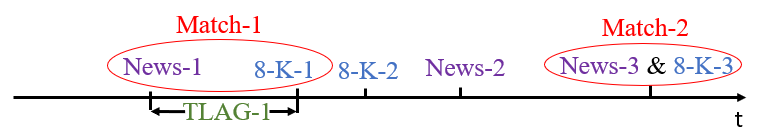
\includegraphics[scale=0.6]{../output/fig/fig1_matching.png}
	\end{center}
\end{figure}

Figuer 1 illustrates the 8-K sample matching process. We match every news day to its first posterior 8-K day, ignoring the successive 8-K days (if any) between two news days (Match-1), or in some cases the 8-K day coincides with news day (Match-2). TLAG is defined as the number of days elapsed between the news release date and 8-K filing date.

%%%%%%%%%%%%%% Figure 2: Sample Selection Process
% Table generated by Excel2LaTeX from sheet 'Fig2'
\begin{table}[htbp] \label{fig2}
  \centering
    \begin{tabular}{lr}
    \multicolumn{2}{c}{Figure 2: Sample Selection Process} \\
    \multicolumn{2}{c}{10-Q} \\
    Numer of observations: &  \\
    Retrieved from EDGAR & 575,579 \\
    After merging with COMP and CRSP data & 190,341 \\
    After merging with I\textbackslash{}B\textbackslash{}E\textbackslash{}S and segment data & 110,114 \\
    After dropping obs. with missing values in key variables and screening & \textbf{91,606} \\
      &  \\
    \multicolumn{2}{c}{8-K} \\
    Numer of observations: &  \\
    Retrieved from EDGAR & 1,489,626 \\
    After merging and matching with COMP and CRSP data & 390,698 \\
    After dropping obs. with missing values in key variables and screening & \textbf{244,401} \\
    After filtering obs. with TLAG smaller or equal to 4 (8-K restricted sample) & \textbf{61,443} \\
    \end{tabular}%
\end{table}%
 \label{fig2}

%%%%%%%%%%%%%% Figure 3: 8-K Item Distribution
\setcounter{figure}{2}
\begin{figure}[htbp]
	\begin{center}
		\caption{8-K Item Distribution} \label{fig3}
		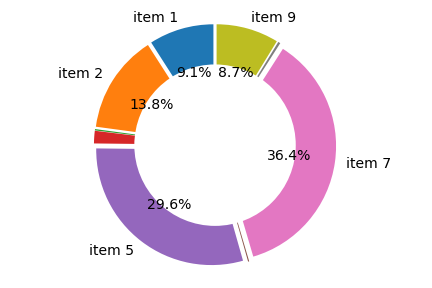
\includegraphics[scale=0.5]{../output/fig/fig3_8-K_before.png}
		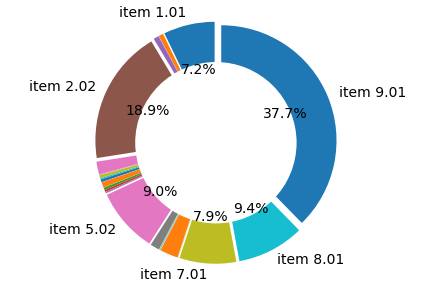
\includegraphics[scale=0.5]{../output/fig/fig3_8-K_after.png}
	\end{center}
\end{figure}

Figuer 3 illustrates the 8-K item distribution before (left) and after (right) August 23rd of 2004. Each share of pie chart shows the percentage of corporate events reported under each 8-K items. See 8-K item list in \hyperref[appd]{Appendix D}.

\newpage
%%%%%%%%%%%%%%%%%%%%%%%%%TABLE 1
\begin{table}[H]
	\centering
	\caption{Constituency Statute' Enactment Years (1975 - 2013)}
	\begin{tabular}{lrrrr}
		\toprule
		\toprule
		State & \multicolumn{1}{l}{Enactment date} & \multicolumn{1}{l}{Before} & \multicolumn{1}{l}{After} & \multicolumn{1}{l}{Total} \\
		\midrule
		AZ    & \multicolumn{1}{l}{07/22/1987} & 57    & 89    & 146 \\
		CT    & \multicolumn{1}{l}{06/07/1988} & 207   & 307   & 514 \\
		FL    & \multicolumn{1}{l}{06/27/1989} & 443   & 756   & 1199 \\
		GA    & \multicolumn{1}{l}{07/01/1989} & 292   & 518   & 810 \\
		HI    & \multicolumn{1}{l}{06/07/1989} & 39    & 52    & 91 \\
		IA    & \multicolumn{1}{l}{12/31/1989} & 95    & 130   & 225 \\
		ID    & \multicolumn{1}{l}{03/22/1988} & 13    & 26    & 39 \\
		IL    & \multicolumn{1}{l}{08/23/1985} & 139   & 277   & 416 \\
		IN    & \multicolumn{1}{l}{04/01/1986} & 261   & 519   & 780 \\
		KY    & \multicolumn{1}{l}{07/15/1988} & 49    & 74    & 123 \\
		LA    & \multicolumn{1}{l}{07/10/1988} & 77    & 114   & 191 \\
		MA    & \multicolumn{1}{l}{07/18/1989} & 687   & 969   & 1656 \\
		MD    & \multicolumn{1}{l}{06/01/1999} & 432   & 352   & 784 \\
		ME    & \multicolumn{1}{l}{09/19/1985} & 74    & 101   & 175 \\
		MN    & \multicolumn{1}{l}{06/01/1987} & 472   & 1,013 & 1485 \\
		MO    & \multicolumn{1}{l}{05/06/1986} & 165   & 306   & 471 \\
		MS    & \multicolumn{1}{l}{07/01/1990} & 2     & 23    & 25 \\
		NC    & \multicolumn{1}{l}{10/01/1993} & 262   & 250   & 512 \\
		NE    & \multicolumn{1}{l}{04/08/1988} & 50    & 32    & 82 \\
		NJ    & \multicolumn{1}{l}{02/04/1989} & 597   & 809   & 1406 \\
		NM    & \multicolumn{1}{l}{04/09/1987} & 30    & 47    & 77 \\
		NV    & \multicolumn{1}{l}{10/01/1991} & 419   & 564   & 983 \\
		NY    & \multicolumn{1}{l}{07/23/1987} & 1,351 & 1,999 & 3350 \\
		OH    & \multicolumn{1}{l}{10/10/1984} & 574   & 1,351 & 1925 \\
		OR    & \multicolumn{1}{l}{03/05/1989} & 134   & 223   & 357 \\
		PA    & \multicolumn{1}{l}{04/27/1990} & 883   & 1,144 & 2027 \\
		RI    & \multicolumn{1}{l}{07/03/1990} & 66    & 110   & 176 \\
		SD    & \multicolumn{1}{l}{07/01/1990} & 27    & 45    & 72 \\
		TN    & \multicolumn{1}{l}{03/11/1988} & 105   & 219   & 324 \\
		TX    & \multicolumn{1}{l}{01/01/2006} & 594   & 241   & 835 \\
		VA    & \multicolumn{1}{l}{03/31/1988} & 341   & 594   & 935 \\
		VT    & \multicolumn{1}{l}{04/16/1998} & 58    & 28    & 86 \\
		WI    & \multicolumn{1}{l}{06/13/1987} & 299   & 559   & 858 \\
		WY    & \multicolumn{1}{l}{01/01/1990} & 32    & 52    & 84 \\
		\midrule
		Total  &       & 9,326 & 13,893 & 23,219 \\
		\bottomrule
		\bottomrule
	\end{tabular}%
	\label{tab:addlabel}%
\end{table}%
\noindent This table presents the enactment dates and number of observations before and after enactment for 34 states out of 35 states that have adopted constituency statutes. North Dakota is excluded because of missing observations before or after law enactment date. Nebraska enacted constituency statute from 1988 to 1995 and from 2007 untill present.

%%%%%%%%%%%%%%%%%%%%%%%%%TABLE 2
\begin{table}[H]
	\centering
	\caption{Basu Summary Statistics (1975-2013)}
	Panel A. Firm-year Observations Before Constituency Statute Law Enactment (N=9,326)
	\begin{tabular}{lrrrrrrrrr}
		\toprule
		\toprule
		& \multicolumn{1}{l}{mean} & \multicolumn{1}{l}{median} & \multicolumn{1}{l}{std. dev.} & \multicolumn{1}{l}{max} & \multicolumn{1}{l}{min} & \multicolumn{1}{l}{p1} & \multicolumn{1}{l}{p25} & \multicolumn{1}{l}{p75} & \multicolumn{1}{l}{p99} \\
		\midrule
		EARN  & 0.088 & 0.098 & 0.151 & 0.378 & -1.034 & -0.524 & 0.049 & 0.163 & 0.378 \\
		RET   & 0.032 & 0.023 & 0.338 & 1.419 & -1.194 & -0.817 & -0.156 & 0.194 & 1.086 \\
		NEG   & 0.466 & 0.000 & 0.499 & 1.000 & 0.000 & 0.000 & 0.000 & 1.000 & 1.000 \\
		SIZE  & 4.310 & 4.144 & 1.953 & 10.388 & 0.623 & 0.623 & 2.841 & 5.636 & 9.264 \\
		BTM   & 0.882 & 0.773 & 0.576 & 3.256 & -0.980 & 0.054 & 0.481 & 1.153 & 3.010 \\
		LEV   & 0.692 & 0.348 & 0.972 & 7.773 & 0.000 & 0.000 & 0.093 & 0.934 & 5.024 \\
		\bottomrule
		\bottomrule
	\end{tabular}%
	\bigbreak
	Panel B. Firm-year Observations After Constituency Statutes Law Enactment (N=13,893)
	\begin{tabular}{lrrrrrrrrr}
		\toprule
		\toprule
		& \multicolumn{1}{l}{mean} & \multicolumn{1}{l}{median} & \multicolumn{1}{l}{std. dev} & \multicolumn{1}{l}{max} & \multicolumn{1}{l}{min} & \multicolumn{1}{l}{p1} & \multicolumn{1}{l}{p25} & \multicolumn{1}{l}{p75} & \multicolumn{1}{l}{p99} \\
		\midrule
		EARN  & 0.025 & 0.060 & 0.162 & 0.378 & -1.034 & -0.820 & 0.023 & 0.086 & 0.290 \\
		RET   & 0.013 & -0.005 & 0.351 & 1.419 & -1.194 & -0.924 & -0.173 & 0.180 & 1.156 \\
		NEG   & 0.509 & 1.000 & 0.500 & 1.000 & 0.000 & 0.000 & 0.000 & 1.000 & 1.000 \\
		SIZE  & 5.589 & 5.628 & 2.261 & 10.388 & 0.623 & 0.790 & 3.875 & 7.245 & 10.388 \\
		BTM   & 0.682 & 0.574 & 0.548 & 3.256 & -0.980 & -0.581 & 0.359 & 0.851 & 2.909 \\
		LEV   & 0.568 & 0.260 & 0.953 & 7.773 & 0.000 & 0.000 & 0.068 & 0.685 & 5.293 \\
		\bottomrule
		\bottomrule
	\end{tabular}%
	\bigbreak
	Panel C. Variable Difference Before and After Contituency Statute Law Enactment
	\begin{tabular}{lcc}
		\toprule
		\toprule
		& \multicolumn{1}{l}{mean difference} & \multicolumn{1}{l}{t-statistic} \\
		\midrule
		EARN  & -0.06*** & -29.76 \\
		RET   & -0.02*** & -4.18 \\
		NEG   & 0.04*** & 6.47 \\
		SIZE  & 1.28*** & 44.61 \\
		BTM   & -0.20*** & -26.79 \\
		LEV   & -0.12*** & -9.60 \\
		\bottomrule
		\bottomrule
	\end{tabular}%
\end{table}%
\noindent This table reports summary statistics for key variables used in Basu measure, separated into two time periods: before (Panel A) and after (Panel B) constituency statute enactment. Panel C demonstrates the differences in mean value between pre-enactment and post-enactment period for all key variables, and the significance of mean differences. EARN, RET, SIZE, BTM and LEV are winsorized at 1 and 99 percentiles. All variables are defined in Appendix B. *, **, and *** indicate significance at 10\%, 5\% and 1\% confidence level respectively.

%%%%%%%%%%%%%%%%%%%%%%%%%TABLE 3
\newgeometry{left=1cm, right=1cm, top=1cm, bottom=1.8cm}
\begin{landscape}
	\begin{table}[H]
		\centering
		\caption{Effect of Constituency Statue Enactments on Conservatism, Three Periods}
		$EARN_{i,t}=\alpha_i+\omega_t+\beta_1RET_{i,t}+\beta_2NEG_{i,t}+\beta_3RET_{i,t}\times NEG_{i,t}+\epsilon_{i,t}$ \qquad \qquad \qquad \qquad \qquad \qquad \qquad \qquad \qquad \qquad \qquad \qquad \qquad \qquad (1)
		
		$EARN_{i,t}=\alpha_i+\omega_t+\beta_1RET_{i,t}+\beta_2NEG_{i,t}+\beta_3RET_{i,t}\times NEG_{i,t}+POST_{i,t}\times (\beta_4+\beta_5RET_{i,t}+\beta_6NEG_{i,t}+\beta_7RET_{i,t}\times NEG_{i,t})+\epsilon_{i,t}$ (2)
		
		$\beta_j=\sum_{K}^{}\delta_{j,k}State_k+\sum_{M}^{}\theta_{j,m}Year_m \qquad j=1,2,3$ \qquad \qquad \qquad \qquad \qquad \qquad \qquad \qquad \qquad \qquad \qquad \qquad \qquad \qquad \qquad \qquad \qquad \quad (3)
		
		\begin{tabular}{lccccccc}
			\toprule
			\toprule
			Dependent Variable: EARN & Baseline Basu & \multicolumn{2}{c}{DiD: 1975-2013} & \multicolumn{2}{c}{1984-1992} & \multicolumn{2}{c}{1985-1990} \\
			& I     & II & III & IV & V& VI & VII \\
			&  &  & Incorp. = State &  & Incorp. = State&  & Incorp. = State\\
			\midrule
			RET   & 0.0603*** &       &       &       &       &       &  \\
			& 6.82  &       &       &       &       &       &  \\
			NEG   & 0.0019 &       &       &       &       &       &  \\
			& 0.70  &       &       &       &       &       &  \\
			\rowcolor[rgb]{ .851,  .851,  .851} RET $\times$ NEG & 0.1171*** &       &       &       &       &       &  \\
			\rowcolor[rgb]{ .851,  .851,  .851}       & 10.07 &       &       &       &       &       &  \\
			POST  &       & -0.006 & 0.0067 & -0.0204 & -0.0029 & -0.0098 & 0.0213 \\
			&       & -0.93 & 0.87  & -1.46 & -0.15 & -0.68 & 1.06 \\
			\rowcolor[rgb]{ .851,  .851,  .851} POST $\times$ RET &       & -0.0114 & -0.0334 & 0.0896 & 0.0508 & 0.0762 & -0.0312 \\
			\rowcolor[rgb]{ .851,  .851,  .851}       &       & -0.37 & -1.07 & 1.18  & 0.49  & 0.87  & -0.26 \\
			POST $\times$ NEG &       & 0.0035 & 0.0091 & -0.0012 & -0.0092 & -0.0133 & -0.0377 \\
			&       & 0.35  & 0.90  & -0.07 & -0.45 & -0.47 & -1.38 \\
			\rowcolor[rgb]{ .851,  .851,  .851} POST $\times$ RET $\times$ NEG &       & 0.1041* & 0.1961*** & 0.0109 & 0.0055 & 0.0421 & 0.0833 \\
			\rowcolor[rgb]{ .851,  .851,  .851}       &       & 2.05  & 4.37  & 0.09  & 0.04  & 0.36  & 0.60 \\
			Constant & 0.1597*** & 0.0644** & 0.0571** & 0.0277 & 0.0171 & 0.0442** & 0.0127 \\
			& 17.27 & 3.45  & 2.77  & 1.53  & 0.87  & 2.80 & 0.64 \\
			Year Fixed Effects (Main) & YES   & YES   & YES   & YES   & YES   & YES   & YES \\
			Firm Fixed Effects (Main) & YES   & YES   & YES   & YES   & YES   & YES   & YES \\
			Year Fixed Effects (Basu Coefficients) & NO    & YES   & YES   & YES   & YES   & YES   & YES \\
			State Fixed Effects (Basu Coefficients) & NO    & YES   & YES   & YES   & YES   & YES   & YES \\
			S.E. Clustered by States & YES   & YES   & YES   & YES   & YES   & YES   & YES \\
			Observations  & 23,219 &                  23,219  &                  17,347  &                     7,202  &                     5,314  &                     4,806  &                    3,514  \\
			Adj. R-square & 0.2970 & 0.3108 & 0.3229 & 0.3645 & 0.3716 & 0.3916 & 0.3950 \\
			\bottomrule
			\bottomrule
		\end{tabular}%
	\end{table}%
	
	\noindent This table reports results of baseline Basu measure (Equation 1) over full sample period (Column I), and DiD results (Equation 2 and 3) in three sample periods: 1975 - 2013 (Column II, III), 1984 - 1992 (Column IV, V) and 1985 - 1990 (Column VI, VII). Column III, Column V and Column VII show the DiD results using only firms that headquarter in their state of incorporation. All variables are defined in Appendix B. EARN and RET are winsorized at 1 and 99 percentiles. All regressions control for firm and year fixed effects. DiD regressions control for Basu coefficient fixed effects. Standard errors are clustered at state of incorporation level. %The Basu coefficient fixed effects absorb slope coefficients in baseline Basu model so they are omitted.  *, **, and *** indicate significance at 10\%, 5\% and 1\% confidence level respectively. T-statistics are reported below coefficients.
	
\end{landscape}
\restoregeometry

%\begin{table}[H]
%\centering
%\caption{Basu Measure of Conditional Conservatism}
%$EARN_{i,t}=\alpha_i+\omega_t+\beta_1RET_{i,t}+\beta_2NEG_{i,t}+\beta_3RET_{i,t}\times NEG_{i,t}+\epsilon_{i,t}$
%\begin{tabular}{lccc}
%\toprule
%\toprule
%Dep. Var. EARN & Prediction & 1975-2013 & 1985-1990 \\
%\midrule
%Constant &       & 0.1597*** & 0.0681*** \\
%&       & 17.27 & 12.54 \\
%RET   &       & 0.0603*** & 0.0793** \\
%&       & 6.82  & 2.84 \\
%NEG   &       & 0.0019 & 0.0087 \\
%&       & 0.70  & 1.21 \\
%\rowcolor[rgb]{ .851,  .851,  .851} RET $\times$ NEG & (+)   & 0.1171*** & 0.0932* \\
%\rowcolor[rgb]{ .851,  .851,  .851}       &       & 10.07 & 2.71 \\
%Year Fixed Effects  &       & YES   & YES \\
%Firm Fixed Effects &       & YES   & YES \\
%S.E. Clustered by States &       & YES   & YES \\
%Observations     &       & 23,219 & 4,806 \\
%Adj. R-square &       & 0.2970 & 0.3781 \\
%\bottomrule
%\bottomrule
%\end{tabular}%
%\end{table}%
%
%%%%%%%%%%%%%%%%TABLE 4
%\begin{table}[H]
%\centering
%\caption{DiD: Effect of Constituency Statue Enactments on Conservatism, Two Periods}
%
%$EARN_{i,t}=\alpha_i+\omega_t+\beta_1RET_{i,t}+\beta_2NEG_{i,t}+\beta_3RET_{i,t}\times NEG_{i,t}+POST_{i,t}\times (\beta_4+\beta_5RET_{i,t}+\beta_6NEG_{i,t}+\beta_7RET_{i,t}\times NEG_{i,t})+\epsilon_{i,t}$
%
%\begin{tabular}{lcccc}
%\toprule
%\toprule
%Dep. Var. EARN & \multicolumn{2}{c}{1975-2013} & \multicolumn{2}{c}{1985-1990} \\
%& I & II& III & IV\\
%& Full & Incorp.=State & Full & Incorp.=State\\
%\midrule
%POST  & -0.006 & 0.0067 & -0.0098 & 0.0213 \\
%& -0.93 & 0.87  & -0.68 & 1.06 \\
%\rowcolor[rgb]{ .851,  .851,  .851} POST $\times$ RET & -0.0114 & -0.0334 & 0.0762 & -0.0312 \\
%\rowcolor[rgb]{ .851,  .851,  .851}       & -0.37 & -1.07 & 0.87  & -0.26 \\
%POST $\times$ NEG & 0.0035 & 0.0091 & -0.0133 & -0.0377 \\
%& 0.35  & 0.90  & -0.47 & -1.38 \\
%\rowcolor[rgb]{ .851,  .851,  .851} POST $\times$ RET $\times$ NEG & 0.1041* & 0.1961*** & 0.0421 & 0.0833 \\
%\rowcolor[rgb]{ .851,  .851,  .851}       & 2.05  & 4.37  & 0.36  & 0.60 \\
%Constant & 0.0644** & 0.0571** & 0.0442** & 0.0127 \\
%& 3.45  & 2.77  & 2.80   & 0.64 \\
%Year Fixed Effects (Main) & YES   & YES   & YES   & YES \\
%Firm Fixed Effects (Main) & YES   & YES   & YES   & YES \\
%Year Fixed Effects (Basu Coefficients) & YES   & YES   & YES   & YES \\
%State Fixed Effects (Basu Coefficients) & YES   & YES   & YES   & YES \\
%S.E. Clustered by States & YES   & YES   & YES   & YES \\
%Observations  &                  23,219  &                  17,347  &                     4,806  &                     3,514  \\
%Adj. R-square & 0.3108 & 0.3229 & 0.3916 & 0.3950 \\
%\bottomrule
%\bottomrule
%\end{tabular}%
%\end{table}%

%%%%%%%%%%TABLE 4
\begin{landscape}
	\begin{table}[H]
		\centering
		\caption{DiD: Effect of Constituency Statue Enactments on Conservatism, Rolling Windows}
		$EARN_{i,t}=\alpha_i+\omega_t+\beta_1RET_{i,t}+\beta_2NEG_{i,t}+\beta_3RET_{i,t}\times NEG_{i,t}+Dummy_{i,t}\times (\beta_4+\beta_5RET_{i,t}+\beta_6NEG_{i,t}+\beta_7RET_{i,t}\times NEG_{i,t})+\epsilon_{i,t}$
		\begin{tabular}{lcccccc}
			\toprule
			\toprule
			Dep. Var. EARN & I & II & III & IV & V & VI \\
			& -1/+1 &  -1/+1 & -2/+2 & -2/+2 & -3/+3 & -3/+3 \\
			& Full & Incorp.= State & Full & Incorp.= State & Full & Incorp.= State \\
			\midrule
			\rowcolor[rgb]{ .906,  .902,  .902} Dummy $\times$ RET$\times$ NEG & 0.1717 & 0.1257 & 0.1622* & 0.1291 & 0.1358** & 0.1266* \\
			& 2.02  & 1.26  & 2.24  & 1.65  & 2.93  & 2.71 \\
			Dummy & -0.0149 & 0.0124 & 0.0187 & 0.0396 & 0.0005 & 0.016 \\
			& -0.92 & 0.71 & 1.01 & 1.61 & 0.04 & 0.94 \\
			Dummy$\times$RET & 0.024 & -0.0052 & 0.0056 & 0.0015 & -0.0079 & -0.0131 \\
			& 0.47 & -0.08 & 0.16 & 0.03 & -0.29 & -0.32 \\
			Dummy$\times$NEG & -0.0042 & -0.0269 & 0.0085 & -0.0035 & 0.007 & -0.0005 \\
			& -0.15 & -0.68 & 0.68 & -0.23 & 0.59 & -0.03 \\
			Constant & 0.0235 & 0.0394* & 0.0900*** & 0.1014*** & 0.1364*** & 0.1368*** \\
			& 1.42 & 2.29 & 4.12 & 4.74 & 11.45 & 10.80 \\
			Year Fixed Effects (Main) & Yes & Yes & Yes & Yes & Yes & Yes \\
			Firm Fixed Effects (Main) & Yes & Yes & Yes & Yes & Yes & Yes \\
			S.E. Clustered by States & Yes & Yes & Yes & Yes & Yes & Yes \\
			Observations & 2,220 & 1,612 & 4,241 & 3,093 & 6,134 & 4,492 \\
			Adj. R-squared & 0.4286 & 0.4169 & 0.3923 & 0.3686 & 0.3655 & 0.3543 \\
			\bottomrule
			\bottomrule
		\end{tabular}%
		\label{tab:addlabel}%
	\end{table}%
	
	\noindent This table reports results of rolling window analysis of conservatism (measured by Basu model) in three subsamples that consist of firm-year observations within one-year (-1/+1), two-years (-2/+2) and three-years (-3/+3) window before and after constituency statute enactments in all states that have adopted the law as of 2013. Column II, Column IV and Column VI show the rolling window results using only firms that headquarter in their state of incorporation. \textit{Dummy} is an indicator variable that takes 1 if this firm-year observation is recorded after law enactment, and 0 if before law enactment. The rest of variables are defined in Appendix B. EARN and RET are winsorized at 1 and 99 percentiles. All regressions control for year and firm fixed effects. Standard errors are clustered at state of incorporation level. *, **, and *** indicate significance at 10\%, 5\% and 1\% confidence level, respectively. t-statistics are reported below coefficients.
\end{landscape}

%%%%%%%%%%%%%%%%%%%%%%TABLE 5
\newgeometry{left=1cm, right=1cm, top=1.7cm, bottom=2cm}
\begin{table}[H]
	\centering
	\caption{Mechanism (1975 - 2013)}                                                 
	\begin{flushleft}
		$EARN_{i,t}=\alpha_i+\omega_t+\beta_1RET_{i,t}+\beta_2NEG_{i,t}+\beta_3RET_{i,t}\times NEG_{i,t}+POST_{i,t}\times (\beta_4+\beta_5RET_{i,t}+\beta_6NEG_{i,t}+\beta_7RET_{i,t}\times NEG_{i,t})+MEC\times(\beta_8RET_{i,t}+\beta_9NEG_{i,t}+\beta_{10}REG_{i,t}\times NEG_{i,t})+MEC\times POST_{i,t}\times (\beta_{11}+\beta_{12}RET_{i,t}+\beta_{13}NEG_{i,t}+\beta_{14}RET_{i,t}\times NEG_{i,t})+\epsilon_{i,t}$ \qquad \qquad \qquad \qquad \qquad \qquad \qquad \qquad \qquad \qquad \qquad(4)
	\end{flushleft}
	\begin{tabular}{lccc}
		\toprule
		\toprule
		Dep. Var. EARN & DCD1 & DCD2 & MA \\
		\midrule
		POST  & 0.0003 & -0.0056 & -0.0160* \\
		& 0.05  & -0.86 & -2.15 \\
		POST$\times$ RET & 0.0112 & -0.0150 & 0.0254 \\
		& 0.38  & -0.47 & 0.81 \\
		POST$\times$NEG & 0.0000 & -0.0022 & 0.0129 \\
		& 0.00  & -0.22 & 1.13 \\
		\rowcolor[rgb]{ .851,  .851,  .851} POST$\times$RET$\times$NEG & -0.0657 & 0.0316 & 0.0709 \\
		\rowcolor[rgb]{ .851,  .851,  .851}       & -1.43 & 0.61  & 1.23 \\
		MEC$\times$RET & 0.0103 & 0.0158 & 0.7419*** \\
		& 0.59  & 1.84  & 4.53 \\
		MEC$\times$NEG & -0.0039 & -0.0024 & 0.1201** \\
		& -0.36 & -0.37 & 2.98 \\
		MEC$\times$RET$\times$NEG & -0.1059* & -0.0700* & -1.5956*** \\
		& -2.46 & -2.34 & -4.21 \\
		MEC$\times$POST & -0.0100 & -0.0220* & 0.1592*** \\
		& -1.31 & -2.47 & 6.14 \\
		MEC$\times$POST$\times$RET & -0.0581* & -0.0562*** & -0.7353*** \\
		& -2.33 & -3.61 & -3.84 \\
		MEC$\times$POST$\times$NEG & 0.0023 & -0.0105 & -0.1559** \\
		& 0.18  & -0.79 & -2.80 \\
		\rowcolor[rgb]{ .851,  .851,  .851} MEC$\times$POST$\times$RET$\times$NEG & 0.2854*** & 0.1751*** & 1.1218* \\
		\rowcolor[rgb]{ .851,  .851,  .851}       & 7.74  & 4.90  & 2.65 \\
		Constant & 0.0609** & 0.0599** & 0.0742*** \\
		& 3.17  & 2.88  & 3.73 \\
		Year Fixed Effects (Main) & YES   & YES   & YES \\
		Firm Fixed Effects (Main) & YES   & YES   & YES \\
		Year Fixed Effects (Basu Coefficients) & YES   & YES   & YES \\
		State Fixed Effects (Basu Coefficients) & YES   & YES   & YES \\
		S.E. Clustered by States & YES   & YES   & YES \\
		Observations    & 23219 & 23219 & 18277 \\
		Adj. R-squared & 0.318 & 0.3334 & 0.2836 \\
		\bottomrule
		\bottomrule
	\end{tabular}%
\end{table}%
\noindent This table reports results of Equation (4): earnings on baseline Basu factors (i.e., NEG, RET, NEG $\times$ RET) and their interactions with POST dummy and three mechanism variables (DCD1, DCD2 and MA). All variables are defined in Appendix B. EARN and RET are winsorized at 1 and 99 percentiles. All regressions control for main firm and year fixed effects and Basu coefficient fixed effects. Standard errors are clustered at state of incorporation level. The Basu coefficient fixed effects absorb slope coefficients in baseline Basu model so they are omitted.  *, **, and *** indicate significance at 10\%, 5\% and 1\% confidence level respectively. T-statistics are reported below coefficients.

\restoregeometry

%%%%%%%%%%%%%%%%%%%TABLE 6
\begin{table}[H]
	\centering
	\caption{KLD Indexes (1995 - 2013)}
	
	Panel A. KLD Summary Statistics
	\begin{tabular}{lrrrrrrrrrr}
		\toprule
		\toprule
		& \multicolumn{1}{l}{N} & \multicolumn{1}{l}{mean} & \multicolumn{1}{l}{median} & \multicolumn{1}{l}{std. dev.} & \multicolumn{1}{l}{max} & \multicolumn{1}{l}{min} & \multicolumn{1}{l}{p1} & \multicolumn{1}{l}{p25} & \multicolumn{1}{l}{p75} & \multicolumn{1}{l}{p99} \\
		\midrule
		KLD\_STR & 12341 & 0.476 & 0     & 1.060 & 12    & 0     & 0     & 0     & 1     & 5 \\
		KLD\_CON & 13922 & 1.011 & 1     & 1.518 & 13    & 0     & 0     & 0     & 1     & 7 \\
		KLD\_TOTAL & 12341 & -0.515 & 0     & 1.403 & 8     & -9    & -5    & -1    & 0     & 3 \\
		Enviroment & 15800 & 0.137 & 0     & 0.427 & 4     & 0     & 0     & 0     & 0     & 2 \\
		Community & 15624 & 0.147 & 0     & 0.476 & 5     & 0     & 0     & 0     & 0     & 2 \\
		Product & 15624 & 0.071 & 0     & 0.272 & 3     & 0     & 0     & 0     & 0     & 1 \\
		Emloyee relation & 12341 & 0.241 & 0     & 0.571 & 5     & 0     & 0     & 0     & 0     & 2 \\
		Human rights & 12986 & 0.003 & 0     & 0.054 & 1     & 0     & 0     & 0     & 0     & 0 \\
		\bottomrule
		\bottomrule
	\end{tabular}%
	
	\bigbreak
	Panel B. KLD Indexes Correlation Matrix
	\begin{tabular}{lrrrrrrrr}
		\toprule
		\toprule
		& KLD\_STR & KLD\_CON & KLD\_TOTAL & Env. & Com. & Prod. & Emp. & Hum.\\
		\midrule
		KLD\_STR & 1.000 &       &       &       &       &       &       &  \\
		KLD\_CON & 0.425 & 1.000 &       &       &       &       &       &  \\
		KLD\_TOTAL & 0.309 & -0.730 & 1.000 &       &       &       &       &  \\
		Enviroment & 0.655 & 0.331 & 0.122 & 1.000 &       &       &       &  \\
		Community & 0.662 & 0.305 & 0.174 & 0.264 & 1.000 &       &       &  \\
		Product & 0.500 & 0.116 & 0.235 & 0.204 & 0.149 & 1.000 &       &  \\
		Employee relation & 0.801 & 0.307 & 0.282 & 0.306 & 0.287 & 0.256 & 1.000 &  \\
		Human rights & 0.145 & 0.043 & 0.062 & 0.023 & 0.117 & 0.031 & 0.064 & 1.000 \\
		\bottomrule
		\bottomrule
	\end{tabular}%
\end{table}%
\noindent This table reports summary statistics (Panel A) and correlation matrix (Panel B) of KLD indexes from 1995 to 2013. All indexes are defined in Appendix C.

%%%%%%%%%%%%%%%%%%TABLE 7
\newgeometry{left=1cm, right=1cm, top=2cm, bottom=2cm}
\begin{landscape}
	\begin{table}[H]
		\centering
		\caption{Association between KLD Indexes and Conservatism , Measured by C\textunderscore Score (1995 - 2013)}
		
		$Conservatism_{i,t}=a_i+b_t+c\times KLD\textunderscore INDEX+d\times X_{i,t}+\epsilon_{i,t}$ \qquad (8)
		
		\begin{tabular}{lccccccc}
			\toprule
			\toprule
			Dependent Variable: C\_Score & I     & II    & III   & IV    & V     & VI    & VII \\
			\midrule
			KLD\_STR & \cellcolor[rgb]{ .906,  .902,  .902}0.0030*** & \cellcolor[rgb]{ .906,  .902,  .902} & \cellcolor[rgb]{ .906,  .902,  .902} & \cellcolor[rgb]{ .906,  .902,  .902} & \cellcolor[rgb]{ .906,  .902,  .902} & \cellcolor[rgb]{ .906,  .902,  .902} & \cellcolor[rgb]{ .906,  .902,  .902}              \\
			& \cellcolor[rgb]{ .906,  .902,  .902}4.95 & \cellcolor[rgb]{ .906,  .902,  .902} & \cellcolor[rgb]{ .906,  .902,  .902} & \cellcolor[rgb]{ .906,  .902,  .902} & \cellcolor[rgb]{ .906,  .902,  .902} & \cellcolor[rgb]{ .906,  .902,  .902} & \cellcolor[rgb]{ .906,  .902,  .902} \\
			KLD\textunderscore TOTAL   & \cellcolor[rgb]{ .906,  .902,  .902} & \cellcolor[rgb]{ .906,  .902,  .902}-0.0011* & \cellcolor[rgb]{ .906,  .902,  .902} & \cellcolor[rgb]{ .906,  .902,  .902} & \cellcolor[rgb]{ .906,  .902,  .902} & \cellcolor[rgb]{ .906,  .902,  .902} & \cellcolor[rgb]{ .906,  .902,  .902} \\
			& \cellcolor[rgb]{ .906,  .902,  .902} & \cellcolor[rgb]{ .906,  .902,  .902}-2.07 & \cellcolor[rgb]{ .906,  .902,  .902} & \cellcolor[rgb]{ .906,  .902,  .902} & \cellcolor[rgb]{ .906,  .902,  .902} & \cellcolor[rgb]{ .906,  .902,  .902} & \cellcolor[rgb]{ .906,  .902,  .902} \\
			Environment & \cellcolor[rgb]{ .906,  .902,  .902} & \cellcolor[rgb]{ .906,  .902,  .902} & \cellcolor[rgb]{ .906,  .902,  .902}-0.0019 & \cellcolor[rgb]{ .906,  .902,  .902} & \cellcolor[rgb]{ .906,  .902,  .902} & \cellcolor[rgb]{ .906,  .902,  .902} & \cellcolor[rgb]{ .906,  .902,  .902} \\
			& \cellcolor[rgb]{ .906,  .902,  .902} & \cellcolor[rgb]{ .906,  .902,  .902} & \cellcolor[rgb]{ .906,  .902,  .902}-1.93 & \cellcolor[rgb]{ .906,  .902,  .902} & \cellcolor[rgb]{ .906,  .902,  .902} & \cellcolor[rgb]{ .906,  .902,  .902} & \cellcolor[rgb]{ .906,  .902,  .902} \\
			Community & \cellcolor[rgb]{ .906,  .902,  .902} & \cellcolor[rgb]{ .906,  .902,  .902} & \cellcolor[rgb]{ .906,  .902,  .902} & \cellcolor[rgb]{ .906,  .902,  .902}-0.0020* & \cellcolor[rgb]{ .906,  .902,  .902} & \cellcolor[rgb]{ .906,  .902,  .902} & \cellcolor[rgb]{ .906,  .902,  .902} \\
			& \cellcolor[rgb]{ .906,  .902,  .902} & \cellcolor[rgb]{ .906,  .902,  .902} & \cellcolor[rgb]{ .906,  .902,  .902} & \cellcolor[rgb]{ .906,  .902,  .902}-2.45 & \cellcolor[rgb]{ .906,  .902,  .902} & \cellcolor[rgb]{ .906,  .902,  .902} & \cellcolor[rgb]{ .906,  .902,  .902} \\
			Product & \cellcolor[rgb]{ .906,  .902,  .902} & \cellcolor[rgb]{ .906,  .902,  .902} & \cellcolor[rgb]{ .906,  .902,  .902} & \cellcolor[rgb]{ .906,  .902,  .902} & \cellcolor[rgb]{ .906,  .902,  .902}0.0060* & \cellcolor[rgb]{ .906,  .902,  .902} & \cellcolor[rgb]{ .906,  .902,  .902} \\
			& \cellcolor[rgb]{ .906,  .902,  .902} & \cellcolor[rgb]{ .906,  .902,  .902} & \cellcolor[rgb]{ .906,  .902,  .902} & \cellcolor[rgb]{ .906,  .902,  .902} & \cellcolor[rgb]{ .906,  .902,  .902}2.42 & \cellcolor[rgb]{ .906,  .902,  .902} & \cellcolor[rgb]{ .906,  .902,  .902} \\
			Employee Relation & \cellcolor[rgb]{ .906,  .902,  .902} & \cellcolor[rgb]{ .906,  .902,  .902} & \cellcolor[rgb]{ .906,  .902,  .902} & \cellcolor[rgb]{ .906,  .902,  .902} & \cellcolor[rgb]{ .906,  .902,  .902} & \cellcolor[rgb]{ .906,  .902,  .902}0.0028** & \cellcolor[rgb]{ .906,  .902,  .902} \\
			& \cellcolor[rgb]{ .906,  .902,  .902} & \cellcolor[rgb]{ .906,  .902,  .902} & \cellcolor[rgb]{ .906,  .902,  .902} & \cellcolor[rgb]{ .906,  .902,  .902} & \cellcolor[rgb]{ .906,  .902,  .902} & \cellcolor[rgb]{ .906,  .902,  .902}3.47 & \cellcolor[rgb]{ .906,  .902,  .902} \\
			Human Rights & \cellcolor[rgb]{ .906,  .902,  .902} & \cellcolor[rgb]{ .906,  .902,  .902} & \cellcolor[rgb]{ .906,  .902,  .902} & \cellcolor[rgb]{ .906,  .902,  .902} & \cellcolor[rgb]{ .906,  .902,  .902} & \cellcolor[rgb]{ .906,  .902,  .902} & \cellcolor[rgb]{ .906,  .902,  .902}-0.0059 \\
			& \cellcolor[rgb]{ .906,  .902,  .902} & \cellcolor[rgb]{ .906,  .902,  .902} & \cellcolor[rgb]{ .906,  .902,  .902} & \cellcolor[rgb]{ .906,  .902,  .902} & \cellcolor[rgb]{ .906,  .902,  .902} & \cellcolor[rgb]{ .906,  .902,  .902} & \cellcolor[rgb]{ .906,  .902,  .902}-0.80 \\
			SIZE  & -0.0094*** & -0.0093*** & -0.0114*** & -0.0108*** & -0.0108*** & -0.0095*** & -0.0102*** \\
			& -8.41 & -8.11 & -9.34 & -8.64 & -8.74 & -8.18 & -8.77 \\
			MTB   & 0.0052*** & 0.0052*** & 0.0055*** & 0.0053*** & 0.0054*** & 0.0052*** & 0.0058*** \\
			& 26.27 & 26.17 & 15.15 & 18.34 & 18.19 & 26.28 & 28.29 \\
			LEV   & 0.061*** & 0.061*** & 0.0576*** & 0.0574*** & 0.0574*** & 0.0610*** & 0.0580*** \\
			& 24.19 & 23.88 & 26.32 & 26.55 & 26.48 & 23.99 & 22.85 \\
			Constant & 0.2287*** & 0.2287*** & 0.0176 & 0.0148 & 0.0136 & 0.2295*** & 0.1523*** \\
			& 30.31 & 29.85 & 1.96  & 1.57  & 1.43  & 29.76 & 22.15 \\
			Year fixed effects & YES   & YES   & YES   & YES   & YES   & YES   & YES \\
			Firm Fixed Effects & YES   & YES   & YES   & YES   & YES   & YES   & YES \\
			S.E. Clustered by States & YES   & YES   & YES   & YES   & YES   & YES   & YES \\
			Observations    & 10483 & 10483 & 13920 & 13742 & 13742 & 10483 & 11087 \\
			Adj. R-square & 0.7778 & 0.7776 & 0.778 & 0.7752 & 0.7753 & 0.7776 & 0.7708 \\
			\bottomrule
			\bottomrule
		\end{tabular}%
		\label{tab:addlabel}%
	\end{table}%
	
	\noindent This table reports results of Equation (8): OLS regression model of conservatism (measured by C\textunderscore Score) on KLD indexes. All KLD indexes are defined in Appendix c. All regressions control for firm and year fixed effects. Standard errors are clustered at state of incorporation level. *, **, and *** indicate significance at 10\%, 5\% and 1\% confidence level respectively. T-statistics are reported below coefficients.
	
\end{landscape}
\restoregeometry

%%%%%%%%%%%TABLE 8
\begin{table}[H]
	\centering
	\caption{DiD: Effect  of Constituency Statute Enactments on C\textunderscore Score, Three Periods}
	$Conservatism_{i,t}=a_i+b_t+c\times POST_{i,t}+d\times X_{i,t}+\epsilon_{i,t}$ \qquad (9)
	\begin{tabular}{lccc}
		\toprule
		\toprule
		Dep. Var. C\_Score & 1975 - 2013 & 1984 - 1992 & 1985 - 1990 \\
		& I & II & III \\
		\midrule
		\rowcolor[rgb]{ .906,  .902,  .902} POST  & 0.0046 & 0.0073* & 0.0112* \\
		\rowcolor[rgb]{ .906,  .902,  .902}       & 1.56  & 2.17  & 2.51 \\
		SIZE  & -0.0150*** & -0.0355*** & -0.0441*** \\
		& -8.27 & -12.94 & -8.83 \\
		MTB   & -0.0018 & -0.0051*** & -0.0044* \\
		& -1.64 & -5.83 & -2.73 \\
		LEV   & 0.0633*** & 0.0329*** & 0.0218*** \\
		& 23.07 & 10.45 & 3.99 \\
		Constant & 0.0824*** & 0.1695*** & 0.2749*** \\
		& 8.98  & 12.68 & 11.41 \\
		Year Fixed Effects & YES   & YES   & YES \\
		Firm Fixed Effects & YES   & YES   & YES \\
		S.E. Clustered by States & YES   & YES   & YES \\
		Observations  & 22570 & 6965  & 4644 \\
		Adj. R-square & 0.5016 & 0.5482 & 0.5194 \\
		\bottomrule
		\bottomrule
	\end{tabular}%
\end{table}%

\noindent This table reports DiD regression (Equation 9) results in three sample periods: 1975 - 2013 (Column I), 1984 - 1992 (Column II) and 1985 - 1990 (Column III). All variables are defined in Appendix B. SIZE, MTB and LEV are winsorized at 1 and 99 percentiles. All regressions control for firm and year fixed effects. Standard errors are clustered at state of incorporation level. *, **, and *** indicate significance at 10\%, 5\% and 1\% confidence level respectively. T-statistics are reported below coefficients.

%%%%%%%%%%%%TABLE 9
\begin{table}[H]
	\centering
	\caption{DiD: Effect of Constituency Statute Enactments on C\textunderscore Score, Rolling Windows}
	$Conservatism_{i,t}=a_i+b_t+c\times Dummy_{i,t}+d\times X_{i,t}+\epsilon_{i,t}$
	\begin{tabular}{lccc}
		\toprule
		\toprule
		Dep. Var. C\_SCORE & I & II & III \\
		\multicolumn{1}{r}{} & -1/+1 & -2/+2 & -3/+3 \\
		\midrule
		\rowcolor[rgb]{ .906,  .902,  .902} Dummy & 0.0223*** & 0.011 & 0.0083 \\
		\rowcolor[rgb]{ .906,  .902,  .902} & 5.89  & 1.09  & 1.36 \\
		SIZE  & -0.0387** & -0.0303***& -0.0318*** \\
		& -3.03 & -5.74 & -6.92 \\
		MTB   & -0.0032 & -0.0049** & -0.0041** \\
		& -1.02 & -3.26 & -3.56 \\
		LEV   & 0.0164 & 0.0319** & 0.0341*** \\
		& 0.74  & 2.92  & 5.13 \\
		Constant & 0.2184*** & 0.2130*** & 0.1846*** \\
		& 3.80  & 8.03  & 8.11 \\
		Year Fixed Effects & Yes & Yes & Yes \\
		Firm Fixed Effects & Yes & Yes & Yes \\
		S.E. Clustered by States & Yes & Yes & Yes \\
		Observations & 2,144 & 4,105 & 5,941 \\
		Adj. R-squared & 0.6858 & 0.7176 & 0.6896 \\
		\bottomrule
		\bottomrule
	\end{tabular}%
\end{table}%
\noindent This table reports results of rolling window analysis of conservatism (measured by C\textunderscore Score) in three subsamples that consist of firm-year observations within one-year (-1/+1), two-years (-2/+2) and three-years (-3/+3) window before and after constituency statute enactments in all states that have adopted the law as of 2013. \textit{Dummy} is an indicator variable that takes 1 if this firm-year observation is recorded after law enactment, and 0 if before law enactment. The rest of variables are defined in Appendix B. SIZE, MTB and LEV are winsorized at 1 and 99 percentiles. All regressions control for year and firm fixed effects. Standard errors are clustered at state of incorporation level. *, **, and *** indicate significance at 10\%, 5\% and 1\% confidence level, respectively. t-statistics are reported below coefficients.

\newpage
\section*{Appendix}
\subsection*{Appendix A: 10-Q and 8-K parsing}
\label{appa}
We develop a Python program to automatically parse, process and retrieve 10-K and 8-K filings from EDGAR database. Our algorithm consists of the following steps:

1. Download all quarterly master indexes from EDGAR using \textit{python-edgar}\footnote{Python-edgar package documentation available at \url{https://github.com/edouardswiac/python-edgar/blob/master/README.md}} package.

2. Filter all 10-Q and 8-K filings\footnote{Our analysis exclude amendments such as 10-Q/A and 8-K/A} from EDGAR master index files and obtain url of the \textit{filing detail} webpage\footnote{One example of filing detail webpage is available at \url{https://www.sec.gov/Archives/edgar/data/320193/000032019320000050/0000320193-20-000050-index.html}} for each of the 10-Q and 8-K filings. 

3. Extract (a) identification information\footnote{For example cik, accession number, reporting period, filing date and 8-K items etc.} and (b) url of report in HTM/TXT format\footnote{One example of report in HTM format is available at \url{https://www.sec.gov/Archives/edgar/data/320193/000032019320000050/a8-kq220203282020.htm}. We first search for url of main report in HTM format. If HTM format main report is not available, then we extract the url of TXT format full report. Each EDGAR filing can be accessed in three formats at maximum: regular text (*.txt), web pages (*.htm) and eXtensible Business Reporting Language, also known as XBRL (*.xml). Early filings in EDGAR are only in TXT format. Later filings extend to HTM format, and in 2009 SEC adopted the XBRL for all corporate filings \cite{secFinalRuleInteractive2009}. Therefore, current existing EDGAR filings all contain a TXT file, and depending on their filing date and company reporting policy they may or may not contain HTM or XML files. Normally all filings in XML format are also available in HTM format. We manually checked 100 random filings that are in XML format, and all of them are also available in HTM format with the same content. The TXT files usually contain not only the main report, but also all other additional filing materials (if any) such as graphics, exhibits and press release etc. However, the HTM files only contain the main report. We mainly focus on HTM files other than TXT files because the former naturally filters out less relevant information, and provides a cleaner textual content of the essential information. XML files are not parsed due to low tractability. } from the \textit{filing detail} webpage for each of the 10-Q and 8-K filings. 

4. Parse and cleanse\footnote{Cleansing steps are: (a) delete nondisplay section; (b) delete all tables that contains more than 4 numbers; and (c) delete all HTML tags} all 10-Q and 8-K filings with url of HTM/TXT format report, using \textit{beautiful soup}\footnote{Beautiful soup package documentation available at \url{https://www.crummy.com/software/BeautifulSoup/bs4/doc/}} package. 

5. Save all clean 10-Q and 8-K filings to local device. 

6. Perform word count on clean 10-Q and 8-K filings using LM dictionary.\footnote{LM dictionary available at \url{https://sraf.nd.edu/textual-analysis/resources/\#LM\%20Sentiment\%20Word\%20Lists}}

All Python scripts and data are available online via \url{https://github.com/fengzhi22/narrative_conservatism}.

\subsection*{Appendix B: Textual Variable Definition}
\label{appb}
\begin{table}[H]
	\centering
	\begin{tabular}{lp{15cm}p{15cm}}
		\textbf{Variable} & \textbf{Definition} \\
		NW & Number of words, defined as the natural logarithm of one plus the count of total words (nw)\\
		nw & Raw count of total words\\
		TONE & Tone, defined as number of net positive words per thousand total words, calculated as total number of positive words minus the sum of total number of negative words and total number of negations, and multiply the previous result by one thousand\\
		TLAG & Time lag, defined as number of days elapsed between the news release date (CRSP entry date) and document filing date (EDGAR filing date)\\
		ABTONE & Abnormal tone, calculated as the residual of the cross-sectional expected tone model (Equation 3)\\
		N8K & Number of 8-Ks reported in one day\\
		NITEM & Number of 8-K items reported in one day\\
		
	\end{tabular}%
\end{table}%

\subsection*{Appendix C: Financial Variable Definition}
\label{appc}
\begin{table}[H]
	\centering
	\begin{tabular}{lp{15cm}p{15cm}}
		\textbf{Variable} & \textbf{Definition} \\
		
		EARN & Quarterly earnings, defined as quarterly earnings before extraordinary items (Compustat data item IBQ) scaled by beginning-of-quarter total assets (Compustat data item ATQ) \\
		$\Delta$EARN & Change in quarterly earnings, defined as current quarterly earnings minus one-quarter-lagged quarterly earnings \\
		LEV & Leverage ratio, defined as beginning-of-quarter short term debt (Compustat data item DLCQ) plus beginning-of-quarter long term debt (Compustat data item DLTTQ) scaled by beginning-of-quarter total assets (Compustat data item ATQ) \\
		MTB & Market-to-book ratio, defined as beginning-of-quarter market value of equity, calculated as common share price (Compustat data item PRCCQ) times common shares outstanding (Compustat data item CSHOQ) divided by beginning-of-quarter book value of equity (Compustat data item CEQQ) \\
		SIZE & Firm size, defined as the natural logarithm of market value of equity, calculated as natural logarithm of common share price (Compustat data item PRCCQ) times common shares outstanding (Compustat data item CSHOQ) \\
		QRET & Quarterly market-adjusted stock return, defined as buy-and-hold stock return (CRSP data item RET) over the fiscal quarter adjusted by the value-weighted stock return (CRSP data item VWRETD) over the same period \\
		DRET & Daily market-adjusted stock return, defined as daily buy-and-hold stock return (CRSP data item RET) adjusted by the daily value-weighted stock return (CRSP data item VWRETD)\\
		$\Delta$DRET & Change in daily market-adjusted stock return (DRET), defined as current daily market-adjusted stock return minus one-day-lagged daily market-adjusted stock return \\
		NEG & Indicator for negative quarterly return, which is set to 1 when market-adjusted stock return (QRET) is negative and 0 otherwise \\
		BN & Indicator for daily bad news, which is set to 1 (0) if the negative (positive) change in daily market-adjusted stock return ($\Delta$DRET) is three times larger than the firm’s average decrease (increase) in daily return over the calendar year.\\
		AF & Analyst forecast, defined as analysts' mean consensus forecast for one-year-ahead earnings per share, scaled by stock price per share at the end of the fiscal quarter (Compustat data item PRCCQ)\\
		AFE & Analyst forecast error, defined as I/B/E/S earnings per share minus the median of the most recent analysts' forecasts, deflated by stock price per share at the end of the fiscal quarter (Compustat data item PRCCQ)\\
		BUSSEG & Business segment, defined as the natural logarithm of one plus number of business segments, or one if item is missing from Compustat\\
		GEOSEG & Geographical segment, defined as the natural logarithm of one plus number of geographical segments, or one if item is missing from Compustat\\
		AGE & Firm age, defined as the natural logarithm of one plus number of days elapsed since the firm's first entry date in CRSP\\
		STD\_EARN & Standard deviation of quarterly earnings (EARN) over the last five quarters\\
		STD\_QRET & Standard deviation of monthly market-adjusted stock return over all months in the fiscal quarter\\
		LOSS & Indicator for loss, which is set to 1 when quaterly earnings (EARN) is negative and 0 otherwise\\
	\end{tabular}%
\end{table}%

\newpage
\subsection*{Appendix D: 8-K Item List}
\label{appd}
% Table generated by Excel2LaTeX from sheet 'Fig4'

\begin{table}[H]
  \centering
  \begin{small}
    \begin{tabular}{ll}
    \multicolumn{2}{c}{\textbf{8-K Item List Before 2004-08-23}} \\
    Item 1 & Changes in Control of Registrant \\
    Item 2 & Acquisition or Disposition of Assets \\
    Item 3 & Bankruptcy or Receivership \\
    Item 4 & Changes in Registrant's Certifying Accountant \\
    Item 5 & Other Events \\
    Item 6 & Resignation of Registrant's Directors \\
    Item 7 & Financial Statements and Exhibits \\
    Item 8 & Change in Fiscal Year \\
    Item 9 & Regulation FD Disclosure \\
    Item 10 & Amendments to the Registrant's Code of Ethics \\
    Item 11 & Temporary Suspension of Trading Under Registrant's Employee Benefit Plans \\
    Item 12 & Results of Operations and Financial Condition \\
      &  \\
    \multicolumn{2}{c}{\textbf{8-K Item List After 2004-08-23 (included)}} \\
    \textbf{Section 1} & \textbf{Registrant's Business and Operations} \\
    Item 1.01 & Entry into a Material Definitive Agreement \\
    Item 1.02 & Termination of a Material Definitive Agreement \\
    Item 1.03 & Bankruptcy or Receivership \\
    Item 1.04 & Mine Safety - Reporting of Shutdowns and Patterns of Violations \\
    \textbf{Section 2} & \textbf{Financial Information} \\
    Item 2.01 & Completion of Acquisition or Disposition of Assets \\
    Item 2.02 & Results of Operations and Financial Condition \\
    Item 2.03 & Creation of a Direct Financial Obligation or an Obligation under an \\
              & Off-Balance Sheet Arrangement of a Registrant \\
    Item 2.04 & Triggering Events That Accelerate or Increase a Direct Financial Obligation or \\
              & an Obligation under an Off-Balance Sheet Arrangement \\
    Item 2.05 & Costs Associated with Exit or Disposal Activities \\
    Item 2.06 & Material Impairments \\
    \textbf{Section 3} & \textbf{Securities and Trading Markets} \\
    Item 3.01 & Notice of Delisting or Failure to Satisfy a Continued Listing Rule or Standard; Transfer of Listing \\
    Item 3.02 & Unregistered Sales of Equity Securities \\
    Item 3.03 & Material Modification to Rights of Security Holders \\
    \textbf{Section 4} & \textbf{Matters Related to Accountants and Financial Statements} \\
    Item 4.01 & Changes in Registrant's Certifying Accountant \\
    Item 4.02 & Non-Reliance on Previously Issued Financial Statements or a Related Audit Report \\
              & or Completed Interim Review \\
    \textbf{Section 5} & \textbf{Corporate Governance and Management} \\
    Item 5.01 & Changes in Control of Registrant \\
    Item 5.02 & Departure of Directors or Certain Officers; Election of Directors; Appointment of Certain Officers; \\
              & Compensatory Arrangements of Certain Officers \\
    Item 5.03 & Amendments to Articles of Incorporation or Bylaws; Change in Fiscal Year \\
    Item 5.04 & Temporary Suspension of Trading Under Registrant's Employee Benefit Plans \\
    Item 5.05 & Amendment to Registrant's Code of Ethics, or Waiver of a Provision of the Code of Ethics \\
    Item 5.06 & Change in Shell Company Status \\
    Item 5.07 & Submission of Matters to a Vote of Security Holders \\
    Item 5.08 & Shareholder Director Nominations \\
    \textbf{Section 6} & \textbf{Asset-Backed Securities} \\
    Item 6.01 & ABS Informational and Computational Material \\
    Item 6.02 & Change of Servicer or Trustee \\
    Item 6.03 & Change in Credit Enhancement or Other External Support \\
    Item 6.04 & Failure to Make a Required Distribution \\
    Item 6.05 & Securities Act Updating Disclosure \\
    \textbf{Section 7} & \textbf{Regulation FD} \\
    Item 7.01 & Regulation FD Disclosure \\
    \textbf{Section 8} & \textbf{Other Events} \\
    Item 8.01 & Other Events \\
    \textbf{Section 9} & \textbf{Financial Statements and Exhibits} \\
    Item 9.01 & Financial Statements and Exhibits \\
              & 
    \end{tabular}%

\begin{tabular}{l}
8-K item classification regimes before and after August 23 of 2004, adapted from \citeA{secFinalRuleAdditional2004}. \\
Other Events, Regulation FD Disclosure and Results of Operations and Financial Condition are voluntary disclosure items.
\end{tabular}
\end{small}
\end{table}%


\newpage
\begin{small}
\subsection*{Appendix E: 8-K Matching Cases}
We check whether the SEC filings and the market returns movements are triggered by the same corporate events, assuming market efficiency. First, we randomly pick 20 good and bad news events. Next, we read the 8-Ks matched to the news and check if the corporate events depicted in the 8-Ks are in line with the market movements both in terms of direction and magnitude. We find that the 8-K matching cases make economic sense overall. See selected 8-K matching cases below.
\label{appe}
\begin{center}
	\textbf{Good News}
\end{center}
\subsubsection*{Case 1: Entry into a Material Definitive Agreement; TLAG = 3}
Human Genome Sciences, Inc. (CIK = 0000901219) experienced a significant rise in market-adjusted daily stock returns ($\Delta$DRET = 2.76) on July 20 of 2009. On July 23 of 2009, the company filed an 8-Ks with ending reporting period on July 17 of 2009. The 8-K contained Item 1.01: Entry into a Material Definitive Agreement, Item 2.02: Results of Operations and Financial Condition and Item 9.01: Financial Statements and Exhibits. The 8-K stated that ``On July 17, 2009, Human Genome Sciences, Inc. (the `Company') and the Biomedical Advanced Research and Development Authority (`BARDA') of the U.S. Government entered into an amendment of solicitation/modification of contract pursuant to which BARDA exercised its option to purchase an additional 45,000 doses of raxibacumab (ABthrax) for the Strategic National Stockpile, to be delivered over a three-year period beginning near the end of 2009. The Company expects to receive approximately \$151 million in revenues from this award as deliveries are completed".
\subsubsection*{Case 2: Drug Test Results Announcement; TLAG = 2}
Opexa Therapeutics, Inc. (CIK = 0001069308) experienced a significant rise in market-adjusted daily stock returns ($\Delta$DRET = 2.67) on September 8 of 2009. On September 10 of 2009, the company filed an 8-K with ending reporting period on September 8 of 2009, which contained Item 8.01: Other Events and Item 9.01: Financial Statements and Exhibits. This 8-K stated that ``On September 8, 2009, Opexa Therapeutics, Inc. (the `Company') issued a press release reporting additional analyses of TERMS data for Tovaxin®, a personalized T-cell immunotherapy for multiple sclerosis (MS)". 
\subsubsection*{Case 3: Sales of Equity Securities; TLAG = 6}
MiddleBrook Pharmaceuticals, Inc. (CIK = 0001161924) experienced a significant rise in market-adjusted daily stock returns ($\Delta$DRET = 1.43) on January 24 of 2008. On January 30 of 2008, the company filed an 8-K with ending reporting period on January 24 of 2008, which contained Item 1.01: Entry into a Material Definitive Agreement, Item 3.02: Unregistered Sales of Equity Securities and Item 9.01: Financial Statements and Exhibits. This 8-K stated that ``On January 24, 2008, Middlebrook Pharmaceuticals, Inc. (the `Company') entered into a Securities Purchase Agreement (the `Securities Purchase Agreement') with selected accredited investors (the `Investors'), to sell an aggregate of approximately 8,750,000 shares (the `Shares') of the Company’s common stock, par value \$0.01 per share (the `Common Stock'), and warrants to purchase an aggregate of approximately 3,500,000 shares of Common Stock (the `Warrant Shares') at an exercise price of \$3.00, subject to certain adjustments (the `Warrants' and, together with the Shares, the `Units'), at a price of \$2.40 per Unit, resulting in gross proceeds to the Company of \$21 million (the 'Offering')".
\subsubsection*{Case 4: Entry into an Agreement; TLAG = 6}
SinoCoking Coal and Coke Chemical Industries, Inc. (CIK = 0001099290) experienced a significant rise in market-adjusted daily stock returns ($\Delta$DRET = 1.38) on September 9 of 2014. On September 15 of 2014, the company filed an 8-K with ending reporting period on September 9 of 2014, which contained Item 8.01: Other Events and Item 9.01: Financial Statements and Exhibits. This 8-K included a press release, which stated that ``SinoCoking Coal and Coke Chemical Industries, Inc. (Nasdaq:SCOK), a vertically-integrated coal and coke processor, today said it has signed an exclusive agreement with both the Institute of Process Engineering of the Chinese Academy of Sciences and the North China Institute of Science and Technology to refine and implement a technology that will be used, beginning next month, to convert the 21 million tons of coal at four SinoCoking underground mines into syngas, a clean burning fuel".
\subsubsection*{Case 5: Sales of Equity Securities; TLAG = 6}
ReWalk Robotics Ltd. (CIK = 0001607962) experienced a significant rise in market-adjusted daily stock returns ($\Delta$DRET = 1.19) on June 5 of 2019. On June 11 of 2019, the company filed an 8-K with ending reporting period on June 5 of 2019, which contained Item 1.01: Entry into a Material Definitive Agreement, Item 3.02: Unregistered Sales of Equity Securities, Item 8.01: Other Events and Item 9.01: Financial Statements and Exhibits. This 8-K stated that ``On June 5, 2019  and June 6, 2019, ReWalk Robotics Ltd. (the `Company') entered into warrant exercise agreements (the `Exercise Agreements') with certain institutional investors (the `Holders') of warrants to purchase the Company’s ordinary shares (the `Public Warrants'), par value NIS 0.25 per share (the `Ordinary Shares'), previously issued in the Company’s follow-on offering in November 2018, pursuant to which the Holders agreed to exercise in cash their Public Warrants to purchase an aggregate of 1,464,665 Ordinary Shares at the existing exercise price of \$7.50 per share, for gross proceeds (before placement agent fees and expenses of approximately \$1 million) to the Company of approximately \$11 million".

\newpage
\begin{center}
	\textbf{Bad News}
\end{center}
\subsubsection*{Case 1: Disposition of Assets; TLAG = 1}
Media Services Group, Inc. (CIK = 0000014280) experienced a significant drop in market-adjusted daily stock returns ($\Delta$DRET = -3.26) on April 13 of 2004. On April 14 of 2004, the company filed an 8-K with ending reporting period on April 14 of 2004, which contained Item 2: Acquisition or disposition of assets. This 8-K stated that ``On March 31, 2004, Media Services Group, Inc. (the `Company') completed its sale of substantially all of the assets relating to its telemarketing sales and teleservices business held by its wholly-owned subsidiary, MKTG Teleservices, Inc. to SD\&A Teleservices, Inc. (`SD\&A'), a Georgia corporation and wholly-owned
subsidiary of the Robert W. Woodruff Arts Center, Inc. for \$3.3 million in cash plus the assumption of certain liabilities relating to such business, subject to
a final working capital adjustment, pursuant to a definitive agreement entered into as of March 31, 2004".
\subsubsection*{Case 2: Termination of a Material Definitive Agreement; TLAG = 0}
Ocean Power Technologies, Inc. (CIK = 0001378140) experienced a significant drop in market-adjusted daily stock returns ($\Delta$DRET = -3.26) on June 2 of 2016. On June 2 of 2016, the company filed two 8-Ks with ending reporting period on the same day, which contained Item 1.02: Termination of a Material Definitive Agreement, Item 1.01: Entry into a Material Definitive Agreement and Item 9.01: Financial Statements and Exhibits. The first 8-K stated that ``On June 2, 2016, Ocean Power Technologies, Inc. (the `Company') and Rodman \& Renshaw, a unit of H. C. Wainwright \& Co., LLC (the `Manager'), agreed to terminate the At the Market Offering Agreement (the `Offering Agreement') dated October 19, 2015, as amended, between the Company and the Manager, relating to the offering and sale of shares of the Company’s common stock, par value \$0.001 per share, having an aggregate offering price of up to \$2,906,836 from time to time through or to the Manager, in an `at the market offering.' The termination of the Offering Agreement is effective immediately and the at the market offering program is no longer available for use by the Company".
\subsubsection*{Case 3: Departure of Directors or Certain Officers; TLAG = 0}
Catuity Inc. (CIK = 0001109740) experienced a significant drop in market-adjusted daily stock returns ($\Delta$DRET = -3.16) on June 22 of 2005. On June 22 of 2005, the company filed an 8-K with ending reporting period on the same day, which contained Item 5.02: Departure of Directors or Certain Officers; Election of Directors; Appointment of Certain Officers: Compensatory Arrangements of Certain Officers. This 8-K stated that ``On Friday June 17, 2005 Catuity learned of the unfortunate and unexpected death of Mr. Alan L. Gilman, one of the Company's members of its Board of Directors. Mr. Gilman died of a heart attack despite having no history of heart trouble". 
\subsubsection*{Case 4: Vote of Security Holders; TLAG = 4}
Biostar Pharmaceuticals, Inc. (CIK = 0001418133) experienced a significant drop in market-adjusted daily stock returns ($\Delta$DRET = -2.19) on June 9 of 2016. On June 13 of 2016, the company filed an 8-K with ending reporting period on June 9 of 2016, which contained Item 5.07: Submission of Matters to a Vote of Security Holders. This 8-K stated that ``On June 9, 2016, Biostar Pharmaceuticals, Inc. (the `Company') held its Annual Meeting of Shareholders at its executive offices in Xianyang City, Shaanxi Province, People's Republic of China. Set forth below are the matters voted upon at the meeting and the voting results. On the record date of April 13, 2016, there were 2,212,188 shares of the Company's common stock issued and outstanding. Proposal 1 (Election of Directors) - The shareholders elected Ronghua Wang, King-fai Leung, Haipeng Wu, Zhongyang Shang and Qinghua Liu as directors of the Company to hold office until the next annual meeting of shareholders and until their successors are duly elected. Proposal 2 (Ratification of Auditors) - The Company's shareholders voted to ratify the appointment of Mazars CPA Limited as the Company's independent registered public accounting firm for the year ending December 31, 2015 with 1,510,989 shares voting for and 25,326 shares voting against (15,431 shares abstaining)".
\subsubsection*{Case 5: Receiving a Request for Clarification from the Stock Exchange; TLAG = 3}
My Size, Inc. (CIK = 0001211805) experienced a significant drop in market-adjusted daily stock returns ($\Delta$DRET = -1.86) on February 14 of 2017. On February 17 of 2017, the company filed an 8-K with ending reporting period on February 14 of 2017, which contained Item 8.01: Other Events and Item 9.01: Financial Statements and Exhibits. This 8-K stated that ``On February 14, 2017, the Company received a verbal request from the Tel Aviv Stock Exchange to clarify to the public the difficulties which hindered the possibility of transferring the Company's shares from market to market. In response to such request, the Company filed a report which contained the following statement..."
\end{small}

\newpage
\setcounter{page}{1}
\section*{Online Appendix}

%%%%%%%%%%%%%%%%%%%%%%%%% Online Appendix TABLE 1
% Table generated by Excel2LaTeX from sheet 'OAT1'
\begin{table}[htbp] \label{oat1}
  \centering
    \begin{tabular}{lcc}
    \multicolumn{3}{c}{\textbf{Online Appendix. Table 1: Expected Tone}} \\
    \midrule
    \midrule
      & (1) & (2) \\
    Dep. Vars. & tone & tone \\
    \midrule
      &   &  \\
    EARN & 0.0068*** & 0.0011** \\
      & (7.84) & (2.47) \\
    QRET & 0.0001 & 0.0000 \\
      & (0.63) & (0.01) \\
    SIZE &-0.0008*** &-0.0002*** \\
      & (-50.78) & (-3.34) \\
    MTB &0.0001*** &-0.0013*** \\
      & (13.94) & (-4.52) \\
    STD\_QRET & -0.0064*** & 0.0690*** \\
      & (-17.00) & (7.58) \\
    STD\_EARN & -0.0206*** & 0.0000 \\
      & (-23.35) & (-0.05) \\
    AGE & 0.0004*** & -0.0003 \\
      & (14.91) & (-1.63) \\
    BUSSEG & 0.0007*** & -0.0006***\\
      & (8.99) & (-4.44) \\
    GEOSEG & -0.0009*** & 0.0002 \\
      & (-14.07) & (0.79) \\
    LOSS &-0.0033*** &-0.0013*** \\
      & (-42.51) & (-4.48) \\
    $\Delta$EARN & -0.0110*** & -0.0012 \\
      & (-13.66) & (-1.19) \\
    AFE & 0.0060*** & 0.0008*** \\
      & (15.86) & (3.10) \\
    AF & -0.0050*** & -0.0001 \\
      & (-12.21) & (-0.30) \\
    Constant & -0.0049*** & 0.0057*** \\
      & (-22.39) & (7.02) \\
      &   &  \\
    Observations & 91,607 & 14,475 \\
    Adjusted R-squared & 8.56\% & 4.41\% \\
    Year-quarter FE & NO & NO \\
    Firm FE & NO & NO \\
    Industry clustered SE & NO & NO \\
    \bottomrule
    \bottomrule
    \end{tabular}%
\end{table}%

\begin{equation*}
\begin{split}
tone_{i,t}=\beta_0&+\beta_1EARN_{i,t}+\beta_2RET_{i,t}+\beta_3SIZE_{i,t}+\beta_4MTB_{i,t}+\beta_5STD\_EARN_{i,t}\\
&+\beta_6STD\_RET_{i,t}+\beta_7AGE_{i,t}+\beta_8BUSSEG_{i,t}+\beta_9GEOSEG_{i,t}+\beta_{10}LOSS_{i,t}\\
&+\beta_{11}\Delta EARN_{i,t}+\beta_{12}AFE_{i,t}+\beta_{13}AF_{i,t}+\epsilon_{i,t}
\end{split}
\end{equation*}

Online Appendix Table 1 presents regression results of the above Equation (Column 1) in comparison with the expected tone model results in \citet*{huangToneManagement2014} (Column 2). Dependent variable $tone_{i,t}$ is defined as net positive words, and is calculated as total number of positive words minus the sum of total number of negative words and total number of negations, deflated by total words. Independent variables are defined in \hyperref[appc]{Appendix C}. All financial variables except returns are winsorized at 1\% and 99\% level. ***, ** and * indicate significance at the 1\%, 5\% and 10\% levels in a two-tailed test. The coefficient of MTB in Column 1 is consistent with that in Column 2 in terms of sign, because \citet*{huangToneManagement2014} use book-to-market ratio instead of market-to-book ratio in the expected tone model. 


%%%%%%%%%%%%%%%%%%%%%%%%% Online Appendix TABLE 2
\newpage
%\begin{landscape}
% Table generated by Excel2LaTeX from sheet 'OAT3'
\begin{table}[htbp] \label{oat2}
  \centering
    \begin{tabular}{lcrrr}
    \multicolumn{5}{c}{\textbf{Online Appendix. Table 2.}} \\
    \multicolumn{3}{c}{\textbf{Panel A: Mean of Coefficients and Standard Errors from Fiscal Yearly Regressions}} &&\\
    \midrule
    \midrule
    Indep. Vars. & Prediction & Coeff. & S.E. & t-stats \\
    \midrule
    Intercept &   & -0.016 & 0.006 & -2.50 \\
    NEG &   & 0.007 & 0.013 & 0.55 \\
    RET & (+) & -0.051 & 0.031 & -1.66 \\
    RET$\times$SIZE & (+) & 0.012 & 0.006 & 2.20 \\
    RET$\times$MTB & (-) & -0.016 & 0.004 & -4.05 \\
    RET$\times$LEV & (-) & 0.033 & 0.040 & 0.81 \\
    RET$\times$NEG & (+) & 0.235 & 0.067 & 3.53 \\
    RET$\times$NEG$\times$SIZE & (-) & -0.034 & 0.011 & -3.09 \\
    RET$\times$NEG$\times$MTB & (+) & 0.020 & 0.006 & 3.25 \\
    RET$\times$NEG$\times$LEV & (+) & -0.099 & 0.076 & -1.30 \\
    SIZE &   & 0.004 & 0.001 & 4.20 \\
    MTB &   & 0.001 & 0.001 & 1.00 \\
    LEV &   & -0.013 & 0.008 & -1.61 \\
    NEG$\times$SIZE &   & -0.001 & 0.002 & -0.48 \\
    NEG$\times$MTB &   & 0.000 & 0.001 & -0.27 \\
    NEG$\times$LEV &   & 0.002 & 0.015 & 0.10 \\
    \bottomrule
    \bottomrule
    \end{tabular}%
\end{table}%

\begin{table}[htbp]
	\centering
	\begin{tabular}{lrrrrrrrrr}
		\multicolumn{10}{l}{\textbf{Panel B: Summary Statistics of C\_SCORE and G\_SCORE}}  \\
		\midrule
		\midrule
		& \multicolumn{1}{c}{mean} & \multicolumn{1}{c}{median} & \multicolumn{1}{c}{std. dev} & \multicolumn{1}{c}{max} & \multicolumn{1}{c}{min} & \multicolumn{1}{c}{p1} & \multicolumn{1}{c}{p25} & \multicolumn{1}{c}{p75} & \multicolumn{1}{c}{p99} \\
		\midrule
		C\_SCORE & 0.053 & 0.054 & 0.063 & 1.143 & -0.228 & -0.103 & 0.015 & 0.092 & 0.212 \\
		G\_SCORE & -0.008 & -0.008 & 0.031 & 0.188 & -1.314 & -0.091 & -0.023 & 0.009 & 0.067 \\
		\bottomrule
		\bottomrule
	\end{tabular}%
\end{table}%

\setcounter{equation}{2}
\begin{equation}
TEX_{i,t}=\beta_0+\beta_1\Delta DRET_{i,t-tlag}+\beta_2BN_{i,t-tlag}+\beta_3\Delta DRET_{i,t-tlag}\times BN_{i,t-tlag}+\beta_nCONTROLS_{i,t}+\epsilon_{i,t}
\end{equation}

Online Appendix Table 2 presents regression results of Equation (3) using restricted 8-K sample. All observations in restricted 8-K sample are subject to four (five) business day 8-K reporting deadline after (before) May 23rd 2004. TEX represents a vector of textual properties that consists of number of words (NW), tone (TONE) and reporting time lag (TLAG). CONTROLS denotes a vector of control variables including firm size (SIZE), market-to-book ratio (MTB) and leverage ratio (LEV). See \hyperref[appb]{Appendix B} and \hyperref[appc]{Appendix C} for textual and financial variable definitions. All financial variables except returns are winsorized at 1\% and 99\% level. Column 2, 4 and 6 include firm and time fixed effects and standard errors are clustered at industry level identified by 4-digit SIC codes. ***, ** and * indicate significance at the 1\%, 5\% and 10\% levels in a two-tailed test.
%\end{landscape} 

\end{document}

